\chapter{\label{chap:prob}Probability theory}

%
% Visualizations from 
% <http://colah.github.io/posts/2015-09-Visual-Information/>
% may be useful.
%
% Add Simpson paradox, either here, or especially in statistics.


% TODO: an intro - maybe with Chomsky quote.

% Human language is probabilistic.
% This is not to say that, it is random,
% but analyzing (or comprehending) natural languages require making inferences under uncertainty.
% Take the following well-known ambiguous sentence.
% \pex
% \begingl
%   \gla We saw her duck with a telescope.//
% \endgl
% \xe
% This sentence is ambiguous in quite a few ways.%
% \sidenote{Try to list all possible interpretations of the sentence.} 
% However, even without further context,
% humans tend to prefer certain interpretations,
% to the extent that some of the interpretations are difficult to enumerate.
% The best solutions we know for 
% finding the most plausible interpretation of such sentences are 
% based on statistical methods,
% where probability theory plays a very important role.

In this chapter,
we will review some of the basic concepts from the probability theory.
% TODO: detailed listing of what comes next

The concepts introduced in this chapter will be
very important in many of the subjects
we will cover during the course.
Like the other background chapters,
you may skip this chapter if you are familiar with the probability theory.

\section{Axioms of the probability}

Probability is a measure of (un)certainty of an event.
In daily usage,
we often associate some events with some probabilities.
We talk about high- or low-probability events,
or sometimes we express our notion of probability
(loosely) by percentages or odds.

Formally,
we quantify the probability an event
with a number between \num{0} and \num{1}.
An event with probability of \num{0} is impossible,
and an event with probability of \num{1} happens with certainty.
Otherwise, any number in between,
expresses the certainty we associate with the occurrence of the event.
For example,
an event with probability of \num{0.5} is as likely to happen as it may not.

The events we talk about are outcomes of trials
(some sort of experiment or observation).
In general, an event is a set of outcomes.
The set of all possible outcomes of a trial is called its sample space,
and conventionally indicated by the Greek letter omega ($\Omega$).

Formally, probabilities has to follow the following set of axioms.

\begin{enumerate}
  \item $P(E) \in \mathbb{R}$, $P(E) \ge 0$.
    Probability of an event $E$ has to be a positive number.
  \item $P(\Omega) = 1$.
    The probability of all possible outcomes of a trial is one.
    Note that this also means that 
    probability of no event can be larger than $1$.
  \item For two \emph{disjoint} events $E_{1}$ and $E_{2}$, 
    $P(E_{1}\cup{}E_{2}) = P(E_{1}) + P(E_{2})$.
    In general, for $N$ disjoint events.
    $P(E_{1}\cup\ldots\cup E_{N} = \sum_{i=1}^{N} P(E_{i})$.
\end{enumerate}

The above three axioms forms the basis of all probabilistic statements.
The other rules that we will discuss later on can all be derived from these three rules.
Note that these axioms,
hence the probability theory,
defines only how to use or manipulate the probabilities.
It does not specify how to obtain probabilities.
There are different schools of thought that assign probabilities to events
using (somewhat) incompatible ways.
Since uncertainty, hence probability,
plays an important role in any statistical study,
we will encounter some of these differences during the course of this course.

\section{Random variables}

The concept of \term{random variable} is central to the probability theory.
The value of a random variable is subject to uncertainties.%
\footnote{
  Although,
  the value of a \emph{random variable} is not necessarily unpredictable,
  as in the typical daily use of the term `random'.
  Most random variables we study involve some uncertainties,
  but also some regularities or structure that we can exploit
  for making inferences.
  Somewhat surprisingly,
  even some aspects of a `truly random' processes include these tendencies,
  which is very important for machine learning,
  and \emph{statistical inference} in general.
}
The value of a random variable depend on the outcome of a set of random events. 
For example, we are often interested in studying outcomes
of experiments or observations that involve uncertainty such as

\begin{itemize}
  \item height or weight of a person selected (randomly) form a population
  \item length of a randomly chosen corpus
  \item whether an email is spam or not
  \item the first word of a book, or the first word uttered by a baby
\end{itemize}

In this context,
we can think of a random variable as a (well-defined) function
from the set of outcomes ($\Omega$) of an experiment to real numbers.
Clearly,
the outcome of some of these trials are not trivial to express as a real number.
Often, for mathematical convenience,
an arbitrary mapping may used,
e.g., from a set of words to consecutive integers.
However,
some of the useful quantities
(e.g., expected value or variance) does only make sense
for random events for which a meaningful mapping to the (real) numbers exists.
For example, we can define random variables whose values are
words or syntactic representations of sentences (trees),
but, in these cases quantities like mean will not be useful
(What is the average word?).%
\footnote{%
  Technically, a random variable takes real numbers.
  A more correct term used for non-numeric random variables is \emph{random element}.
  We will be using the term random variable for both cases.
}
Note that the values of random variables are not probabilities,
Probabilities are associated with the outcomes of the random experiment.

Mapping some outcomes to numbers is easy,
for example, if we are measuring the frequency of a sound signal,
or counting the number of words in a document,
the measurement already gives us a real value.
The mapping may not be trivial in some other cases,
such as whether the random variable representing
a product review is positive or negative,
or part of speech of a word.
In these cases,
there are often conventional methods for mapping these outcomes to numbers.
For example,
the Boolean variables (such as binary outcome of a review)
are typically mapped to \num{0} and \num{1} for negative and positive outcomes respectively.


For trials having outcomes with more than two categories
(as in our part of speech example),
a possible solution is to map them to integers arbitrarily,
for example,
as on the row labeled `Integer` in Table~\ref{tbl:nominal-repr}.
\begin{table}
  \begin{tabular}{lrrrrr}
    \toprule
    Part of speech            & Noun & Verb  & Adjective  & Adverb & \ldots \\
    \midrule
    Integer       & \num{1} & \num{2}  & \num{3}  & \num{4} & \ldots \\
    Binary vector &\num[minimum-integer-digits=6,group-digits=false]{1}
                  &\num[minimum-integer-digits=6,group-digits=false]{10}
                  &\num[minimum-integer-digits=6,group-digits=false]{100}
                  &\num[minimum-integer-digits=6,group-digits=false]{1000}
                  &\ldots \\
    \bottomrule
  \end{tabular}
  \caption{
    Alternative numeric representations for categorical (nominal) variables.
  }\label{tbl:nominal-repr}%
\end{table}

However, there is another method that is more convenient for many purposes.
Instead,
we map each outcome to a vector of binary (\num{0} or \num{1}) values,
where we set only a particular member of the vector to $1$,
and we set the rest to \num{0} for a particular outcome.
This representation is called \term{one-of-k} or \term{one-hot} representation,
and exemplified on the row labeled `Binary vector' in Table~\ref{tbl:nominal-repr}.
\label{desc:one-hot}
In statistical literature it is also called \term{dummy coding}.%
\footnote{%
  Note that the coding as we describe here is somewhat redundant.
  We can be slightly more economical by mapping
  one of the outcomes to all zeros.
  Although this economy is not really useful for many purposes,
  it is sometimes used (especially in statistics)
  when one of the outcomes is a special base case (coded as all zeros).
  This makes comparison of other outcomes to the base case easier.
}
This particular representation is used quite often in machine learning
while encoding categorical features.
For example whether a particular word (out of all words in a dictionary)
occurs in a document or not.%
\footnote{%
  If the outcomes/items (such as words) represented have some features
  in common,
  we can even use real values (rather than binary one-hot) in these vectors.
  We will later discuss such `dense' representations.
}

In the discussion above,
we implicitly made a distinction between two types of random variables.
Some random variables are continuous,
they can take any real number as values
(such as height or frequency).
Others, on the other hand, have discrete values.
For example,
number of words in a document or sentence can only take integer values,
and whether a document is spam or not can have only two values (true or false).
This distinction between the continuous
and categorical random variables is important, in general,
and in our discussion of some important properties
and specific distributions of random variables below.

To make the discussion more concrete,
we will use an example hypothetical random variable.
Assume that predicting the length of utterances
in a (particular type of) dialog is important for our purposes.
So, our random variable, $X$, is a discrete variable,
taking only integer values (length of utterances).
For simplicity,
we will also assume that the longest possible utterance is \num{11} words.
\begin{margintable}
  \caption{\label{tbl:prob-table}%
    Probabilities of all possible values ($x$)
    of an example random variable $X$ (utterance lengths).
  }
  \begin{center}
    \begin{tabular}{lS[round-precision=3]}
      \toprule
      $x$ & {$P(X = x)$} \\
      \midrule
      1&0.1554647600\\
      2&0.1847803882\\
      3&0.2098059244\\
      4&0.1990806945\\
      5&0.1022471910\\
      6&0.0655771195\\
      7&0.0390194076\\
      8&0.0228804903\\
      9&0.0115423902\\
     10&0.0053115424\\
     11&0.0042900919\\
      \bottomrule
    \end{tabular}
  \end{center}
\end{margintable}
Table~\ref{tbl:prob-table} lists each possible value of $X$,
with its associated probability.
Note that, in our example, $X$ is the random variable,
and $x$ is a possible value.
The first row of Table~\ref{tbl:prob-table} shows the $P(X=1)$,
whose probability turns out to be \num[round-precision=3]{0.1554647600}.
For now, we do not ask where these probabilities come from.%
\footnote{They are \emph{estimated} from a real corpus of spoken language,
but we will delay the details for now.
}
However,
it is important to note that the probabilities in the table sum to $1$
(except for potential rounding error).

In our utterance-length example (in Table~\ref{tbl:prob-table}),
there is a natural mapping between the utterance length
and the value of the random variable.
The value of the random variable is simply the integer
that corresponds to the utterance length in words.
This mapping is not always straightforward.
To demonstrate that we will give another hypothetical example
in Table~\ref{tbl:prob-table-letters}.
\begin{margintable}
  \caption{\label{tbl:prob-table-letters}%
    Probability distribution of variable $X$,
    associated with letter probabilities.
    Note that the mapping between the letters
    and the values of the random variable $x$ is arbitrary.
  }
  \begin{center}
    \begin{tabular}{lSS[round-precision=3]}
      \toprule
      letter & $x$ & {$P(X = x)$} \\
      \midrule
      a & 1&0.2330012\\
      b & 2&0.0424207\\
      c & 3&0.0464163\\
      d & 4&0.0841186\\
      e & 5&0.2859216\\
      f & 6&0.0262472\\
      g & 7&0.0633547\\
      h & 8&0.2185197\\
      \bottomrule
    \end{tabular}
  \end{center}
\end{margintable}
We assume that we are working on an ancient language,
which is written only with eight letters.
The random variable (we will use $X$ again) this time maps
the relationship between the event (observing a particular the letter) and
the value of the random variable ($x$) is more arbitrary

In both examples above,
we specified probability of a particular value of a random variable like $P(X=x)$,
for example $P(X=1)$
in Table~\ref{tbl:prob-table-letters} is \num{0.2330012}.
However, when there is no ambiguity,
we will skip the name of the random variable and write, for example,
$P(1) = \num{0.2330012}$, or even $P(\text{a}) = \num{0.2330012}$.

\subsection{Probability mass function}

\begin{marginfigure}[4ex]
  \tikzsetnextfilename{prob-mass-func},
  \begin{tikzpicture}[x=3.8mm,y=10cm]
    \foreach \x/\y in {1/0.1554647600,
                       2/0.1847803882,
                       3/0.2098059244,
                       4/0.1990806945,
                       5/0.1022471910,
                       6/0.0655771195,
                       7/0.0390194076,
                       8/0.0228804903,
                       9/0.0115423902,
                      10/0.0053115424,
                      11/0.0042900919}%
    {
      \draw[fill=blue!20]
        ($ (\x,0) + (-0.4, 0) $) rectangle ($ (\x,\y) + (0.4, 0) $);
      \node[anchor=north,font=\scriptsize] at (\x, 0) {\x};
      \draw[thick] (0.4,0) -- (0.4, 0.25);
      \foreach \i in {0, 0.05, 0.1, 0.15, 0.20, 0.25}{%
        \draw (0.4,\i) -- ++(-0.2, 0);
      }
      \foreach \i in {0, 0.1, 0.2}{%
        \node[anchor=east,font=\scriptsize] at (0.2,\i) 
          {\num[round-precision=1]{\i}};
      }
    }
  \end{tikzpicture}
  \caption{\label{fig:pmf}Graphical representation of probability mass function defined in Table~\ref{tbl:prob-table}.}
\end{marginfigure}
\emph{Probability mass function} (PMF) is a function that maps
the values of a discrete random variable to their probabilities.
The PMF of a random variable maps all possible values of the random variable
to exact probability of the associated event.
For example, probability of
an utterance of length \num{3} is \num{0.21} in our example (Table~\ref{tbl:prob-table}).
A probability mass function defines a discrete probability distribution.
Table~\ref{tbl:prob-table} defines such a PMF,
which is shown graphically in Figure~\ref{fig:pmf}.

\subsection{Probability density function}

Continuous random variables do not have probability mass functions,
but analogously they can be defined through
a \emph{probability distribution function} (PDF).
For continuous distributions,
the probability of a single value of the random variable is zero.
We can only talk about non-zero probabilities of intervals.
This may be unintuitive at first thought.
However, if you consider the fact that there are infinite number of real numbers
between any arbitrary range $[a, b]$ ($a \ne b$),
probability of any single value is statistically equivalent to zero.

% approximate gamma function declaration from:
% http://tex.stackexchange.com/questions/120441/plot-the-probability-density-function-of-the-gamma-distribution
\begin{marginfigure}
  \tikzsetnextfilename{prob-density}
  \begin{tikzpicture}[
      declare function={%
        gamma(\z)= (2.506628274631*sqrt(1/\z) +%
                    0.20888568*(1/\z)^(1.5) +%
                    0.00870357*(1/\z)^(2.5) -%
                    (174.2106599*(1/\z)^(3.5))/25920 -%
                    (715.6423511*(1/\z)^(4.5))/1244160%
                   )*exp((-ln(1/\z)-1)*\z);
      },
      declare function={%
        gammapdf(\x,\k,\theta) = \x^(\k-1)*exp(-\x/\theta) /%
                                (\theta^\k*gamma(\k));%
      }
  ]

      \begin{axis}[axis lines=left,
          enlargelimits=upper,
          samples=50,
          x=15mm,
          y=20mm,
      ]
          \addplot[smooth, thick, blue, domain=0:2.5,name path=curve]
            {gammapdf(x,3,0.2)};
          \addplot[draw=none, domain=0:2.5,name path=xax] {0};
          \addplot[blue,opacity=0.2]
            fill between[of=curve and xax,soft clip={domain=0:2.5}];
          \addplot[blue,opacity=0.4]
            fill between[of=curve and xax,soft clip={domain=1:1.5}];

      \end{axis}
%        \draw[domain=0:3,smooth,variable=\x]
%                plot (\x,{gammapdf(\x,3,0.2)});
  \end{tikzpicture}
  \caption{\label{fig:pdf}Example probability density function (PDF).
    Area under the whole curve, potentially stretching to infinity,
    is \num{1} units.
    The area under a particular interval is the probability
    that the random variable takes a value within the interval.
  }
\end{marginfigure}
As an example of a continuous random variable,
suppose we were measuring the durations of the utterances
rather than the number of words as in our discrete random variable example,
we cannot assign a non-zero probability to 
an utterance being \SI{1.4}{\second}.
However, we can assign a probability to a range,
say between \SI{1.2}{\second} and \SI{1.6}{\second}.
As a result,
the values of a PDF are not probabilities.
Figure~\ref{fig:pdf} shows a probability density function.
For the sake of demonstration,
we will pretend this to be the distribution of durations of utterances
in a spoken language corpus.
The plot actually shows a well-known density function.
Precisely, this is the probability density function of
the gamma distribution with parameters $k=3$, $\theta=0.2$,
but this is not important for this introduction.
Figure~\ref{fig:pdf} clearly shows that
the values of the PDF are not probabilities.
For example, the value corresponding to \num{0.5} is grater than \num{1}.
Another important property of the PDF,
more difficult measure from the figure,
is that the area under the curve is \num{1} unit.
Although probabilities of individual real numbers are zero,
we can calculate the probabilities of ranges,
like the one highlighted in Figure~\ref{fig:pdf}.
The probability is simply the definite integral of the PDF
in the interval we are interested in.
In this respect,
the PDF has a very similar function to probability mass function.
However,
we should not forget that the values of a PDF are not probabilities.%
\sidenote[][-10ex]{
%  \begin{tcolorbox}[colback=white,colframe=gray,halign=left,width=\linewidth]
    A common convention for distinguishing,
    a PMF from a PDF is using
    uppercase $P()$ for the former and lowercase $p()$ for tha latter.
    $P(X=x)$ yields the probability of discrete random variable being $x$,
    but the values returned by $p()$ are not probabilities,
    although higher values will indicate neighborhoods
    of high probability density.
%  \end{tcolorbox}
}

We will give brief descriptions
of some of the important continuous probability distributions
later in this chapter.

\subsection{Cumulative distribution function}

\begin{margintable}
  \caption{\label{tbl:cdf}%
    The values of \emph{probability mass function} (column 2)
    and  \emph{cumulative distribution function} (column 3)
    of the earlier example random variable, $X$, presented
    in Table~\ref{tbl:prob-table}.
  }
  \begin{center}
    \begin{tabular}{lS[round-precision=3]S[round-precision=3]}
      \toprule
      $x$ & {$P(X = x)$} & {$P(X \le x)$}\\
      \midrule
      1& 0.1554647600 & 0.1554647600\\
      2& 0.1847803882 & 0.3402451482\\
      3& 0.2098059244 & 0.5500510726\\
      4& 0.1990806945 & 0.7491317671\\
      5& 0.1022471910 & 0.8513789581\\
      6& 0.0655771195 & 0.9169560776\\
      7& 0.0390194076 & 0.9559754852\\
      8& 0.0228804903 & 0.9788559755\\
      9& 0.0115423902 & 0.9903983657\\
     10& 0.0053115424 & 0.9957099081\\
     11& 0.0042900919 & 1.0000000000\\
      \bottomrule
    \end{tabular}
  \end{center}
\end{margintable}
\emph{Cumulative distribution function} (CDF),
or \emph{distribution function} of a random variable $X$,
$F_{X}(x)$, yields the probability that $X$ will take a value
less than or equal to $x$.
\[
  F_{X}(x) = P(X \le x)
\]
In case of discrete distributions,
it is simply the sum of probabilities of all values up to and including $x$.
And, for continuous distributions,
it is the area of under the probability density function
in interval $[-\infty, x]$.
As may you have already guessed,
to evaluate the value of the CDF of a continuous random variable,
we need to integrate the PDF in this range
instead of summing.
Output of a CDF is a probability
regardless of whether the random variable is continuous or discrete.
The cumulative distribution function plays an important role
in statistics, particularly in hypothesis testing.

Table~\ref{tbl:cdf} repeats the probability mass function from
Table~\ref{tbl:prob-table} (in column 2),
and also shows the values cumulative distribution function.
Note that the CDF converges to \num[round-precision=1]{1.0}
at the maximum value of the random variable $X$.

\begin{marginfigure}
  \tikzsetnextfilename{porb-cdf}
  \begin{tikzpicture}[x=3.8mm,y=25mm]
    \foreach \x/\y in {1/0.1554647600,
                       2/0.3402451482,
                       3/0.5500510726,
                       4/0.7491317671,
                       5/0.8513789581,
                       6/0.9169560776,
                       7/0.9559754852,
                       8/0.9788559755,
                       9/0.9903983657,
                      10/0.9957099081,
                      11/1.0000000000}%
    {
      \draw[fill=blue!20]
        ($ (\x,0) + (-0.4, 0) $) rectangle ($ (\x,\y) + (0.4, 0) $);
      \node[anchor=north,font=\scriptsize] at (\x, 0) {\x};
      \draw[thick] (0.4,0) -- (0.4, 1);
      \foreach \i in {0, ..., 10}{%
        \draw (0.4,\i/10) -- ++(-0.2, 0);
      }
      \foreach \i in {0, 0.5, 1.0}{%
        \node[anchor=east,font=\scriptsize] at (0.2,\i) 
          {\num[round-precision=1]{\i}};
      }
    }
  \end{tikzpicture}
  \caption{\label{fig:cdf}Graphical representation
  of cumulative distribution function defined in Table~\ref{tbl:cdf}.}
\end{marginfigure}

\subsection{\label{ssec:expected-value}Expected value}

Expected value of a random variable is its arithmetic mean ($\mu$).
Given a list of numbers,
their arithmetic mean is simply their sum divided
by the total number of numbers in the list.
Assume that we have the following numbers,
say as the length of utterances of interest
in a (small) spoken language corpus:
\begin{center}
  \num{1},
  \num{2},
  \num{3}, \num{3}, \num{3},
  \num{4}, \num{4},
  \num{5},
  \num{7},
  \num{11}
\end{center}
To find the arithmetic mean,
we simply sum these numbers up, and divide the number of items in our list.
Which gives us \num[round-precision=1]{4.3}. 
\begin{marginfigure}
  \tikzsetnextfilename{histogram-mean}
  \begin{tikzpicture}[x=4mm,y=5mm]
    \foreach \x/\y in {1/1,
                       2/1,
                       3/3,
                       4/2,
                       5/1,
                       7/1,
                      11/1}%
    {
      \draw[fill=blue!20]
        ($ (\x,0) + (-0.4, 0) $) rectangle ($ (\x,\y) + (0.4, 0) $);
      \node[anchor=north,font=\scriptsize] at (\x, 0) {\x};
      \draw[thick] (0.4,0) -- (0.4, 4);
      \foreach \i in {0, ..., 4}{%
        \draw (0.4,\i) -- ++(-0.2, 0);
        \node[anchor=east,font=\scriptsize] at (0.2,\i) 
          {\num[round-precision=1]{\i}};
      }
      \draw[dashed,thick,orange] (4.3,0) -- (4.3,4) 
        node[very near end,anchor=west] {$\mu = 4.3$};
    }
  \end{tikzpicture}
  \caption{\label{fig:hist-mean}%
    A graphical representation (histogram) of the distribution of the  numbers in the example.
    Dashed orange line marks the mean.
  }
\end{marginfigure}

Rather than a fixed sample as in the example above,
we are interested in the mean of a probability distribution,
defined as a set of numbers with their probabilities,
we calculate the average by weighting each value with its probability.
The mean, or the expected value,
of the probability distribution shown in Table~\ref{tbl:prob-table} is
%TODO: better formatting of the formula
\begin{equation}
  \footnotesize
  \label{eqn:example-exp-val}
  \begin{aligned}
   & 0.155 \times 1 +
    0.185 \times 2 +
    0.210 \times 3 +
    0.194 \times 4 +
    0.102 \times 5 +&\\
   & 0.066 \times 6 +
    0.039 \times 7 +
    0.023 \times 8 +
    0.012 \times 9 +
    0.005 \times 10 +&
    0.004 \times 11 = 3.497\;.\\
  \end{aligned}
\end{equation}
Note that the expected value is not (necessarily) the most likely value.
In our example,
it is not even a value that the random variable can take.
Nevertheless, it is an important quantity
indicating the central tendency of a probability distribution,
and it is often used for characterizing probability distributions.

In plain words, we multiply each value with its probability,
and sum them up.%
%\marginnote{
%  \begin{tcolorbox}[colback=white,colframe=gray,halign=left,width=\linewidth]
%    A sizable minority of (computational) linguistics students
%    tend to be intimidated by mathematical notation,
%    sometimes as basic as the ones on the left.
%    For the current equations,
%    you should note that $\sum$ is nothing more than
%    a compact notation for multiple additions
%    like the one in Equation~\ref{eqn:example-exp-val}.
%    For most mathematical notation and topics needed in this course,
%    you can refer to Chapter~\ref{ch:math} and the pointers provided
%    to more complete/authoritative sources at the end of it.
%  \end{tcolorbox}
%}
The expected value of a discrete random variable is 
\begin{equation}\label{eqn:expected-value}
  E[X] = \sum_{x} P(x) x .
\end{equation}
where $x$ ranges over all values of $X$,
and $P(x)$ is a shorthand for $P(X=x)$,
the probability of a random variable $X$ taking the value $x$
as defined by its probability mass function.
In general, the expected value of a function of a random variable
$E[f(X)]$ can be calculated using,
\begin{equation}\label{eqn:expected-value-function}
  E\left[f(X)\right] = \sum_{x} P(x) f(x) .
\end{equation}
In Equation~\ref{eqn:expected-value} above,
we simply used the identity function $f(x) = x$.

For continuous variables,
we need an infinite sum, so, we integrate rather than sum:
\[
  E\left[f(X)\right] = \int_{-\infty}^{\infty} p(x) f(x) dx
\]
Note that, here, $p(x)$ is the probability density function.

\todo[inline]{Discuss the linearity of expected value.}

\subsection{Median and mode}

Like the expected value,
\emph{median} and \emph{mode} are two other quantities (statistics)
that are useful in characterizing the central tendency of probability distributions.

\begin{marginfigure}
  \tikzsetnextfilename{hist-mean-median-mode}
  \begin{tikzpicture}[x=4mm,y=5mm]
    \foreach \x/\y in {1/1,
                       2/1,
                       3/3,
                       4/2,
                       5/1,
                       7/1,
                      11/1}%
    {
      \draw[fill=blue!20]
        ($ (\x,0) + (-0.4, 0) $) rectangle ($ (\x,\y) + (0.4, 0) $);
      \node[anchor=north,font=\scriptsize] at (\x, 0) {\x};
      \draw[thick] (0.4,0) -- (0.4, 4);
      \foreach \i in {0, ..., 4}{%
        \draw (0.4,\i) -- ++(-0.2, 0);
        \node[anchor=east,font=\scriptsize] at (0.2,\i) 
          {\num[round-precision=1]{\i}};
      }
      \draw[dashed,thick,orange] (4.3,0) -- (4.3,3) 
        node[very near end,anchor=west,font=\scriptsize] {$\mu = 4.3$};
      \draw[dashed,thick,red] (3.5,0) -- (3.5,4.5) 
        node[very near end,anchor=west,font=\scriptsize] {$m = 3.5$};
      \node[blue,anchor=south east,font=\scriptsize]
        (mm) at (3, 4.2) {mode = \num{3}};
      \draw[->,blue] (mm.south) to[bend left] (3,3);
    }
  \end{tikzpicture}
  \caption{\label{fig:hist-mean-median-mode}%
    The histogram in Figure~\ref{fig:hist-mean} repeated.
    This time we also mark median ($m$, red dashed line) and the mode,
    and the mode.
  }
\end{marginfigure}
The \emph{median} of a random variable is the value that splits
the probability mass (or density) into two equal parts.
More formally, for a random variable $X$,
the median is defined as a number $m$ that satisfies
\begin{equation}\label{eqn:median}
  P(X \le m) \ge \frac{1}{2}\quad\text{and}\quad
  P(X \ge m) \ge \frac{1}{2} .
\end{equation}
Going back to our finite sample of numbers,  
  $[$~\num{1},
  \num{2},
  \num{3}, \num{3}, \num{3},
  \num{4}, \num{4},
  \num{5},
  \num{7},
  \num{11}~$]$,
the easiest way to find the median is to find the number that splits the ordered list into two equal halfs.
For odd number of numbers,
this is the number in the middle.
For even number of numbers, as in our case,
median is conventionally defined as the mean of the two middle numbers,
which is \num[round-precision=1]{3.5} for our example.%
\sidenote{Technically any number that satisfies inequalities in (\ref{eqn:median}) is a median,
which is any number between \num{3} and \num{4} (not including).
In general, $m$ is not guaranteed to be unique,
but for the sake of simplicity,
we will continue talking about `the median' of a distribution.

}

Given a probability distribution,
the mode is found simply by solving the inequalities above for $m$.
For example, for a continuous probability distribution,
that would mean solving
\[
  \int_{-\infty}^{m} p(x) f(x) dx \le \frac{1}{2}
\]
for $m$.

The \emph{mode} of a finite sample is the value that occurs most often.
In our example data above,
the most frequent value is \num{3},
so it is the mode (see Figure~\ref{fig:hist-mean-median-mode}).
The mode of a probability distribution is
the value(s) for which probability mass or density function yields
the maximum result.
For discrete distributions,
this is simply the most probable value.
The examples we had so far are \emph{unimodal},
they have only one mode.
However, some distributions can be \emph{bimodal},
or in general, \emph{multimodal}.
A continuous probability distributions is called multimodal,
if there are multiple local maxima
(peaks with possibly different heights),
as in Figure~\ref{fig:multimodal}.
\begin{marginfigure}
  \tikzsetnextfilename{multimodal-distribution}
  \begin{tikzpicture}[
      declare function={%
        normpdf(\x,\m,\s) = exp(-(\x -\m)^2/(2*\s)^2) /%
                                (\s*(2*pi)^0.5);%
      }
  ]
      \begin{axis}[
          axis lines=middle,
          hide y axis,
          enlargelimits=true,
          samples=50,
          x=3mm,
          y=50mm,
          x axis line style={<->}
      ]
          \addplot[smooth, thick, blue, domain=-6:6,name path=curve]
            {(normpdf(x,-2,0.7)+normpdf(x,2,0.6))/2};
          \addplot[draw=none, domain=-6:6,name path=xax] {0};
          \addplot[blue,opacity=0.2]
            fill between[of=curve and xax,soft clip={domain=-6:6}];
      \end{axis}
  \end{tikzpicture}
  \caption{\label{fig:multimodal}%
    An example multimodal (bimodal) continuous probability distribution.
  }
\end{marginfigure}
Multimodal distributions are interesting,
as they often indicate a \emph{confounding} variable.
For example,
distribution of heights or weights of university students are
probably bimodal,
since the differences in gender will result in having
two peaks around the means of males and females.

The \emph{mean}, \emph{median} and \emph{mode} are
measures of central tendency.
The mean is most commonly used measure of central tendency in many tasks in statistics and machine learning,
since it has nice algebraic properties.
However, as you can see in Figure~\ref{fig:hist-mean-median-mode},
mean is affected from extreme values.
Since the distribution in the figure is skewed,
and there are extreme values
(i.e., the effect of \num{11} in the figure is much higher than
the other data points closer to the center),
mean is moved from the center of the distribution
towards these extreme values.
The median is not affected by extreme values,
but it does not have the same nice algebraic properties.
The median is often used in statistics as a robust measure 
(a measure that is not affected by outliers) of central tendency.
The mode is easy to interpret,
but it also lacks the nice algebraic properties of mean.
Furthermore, mode is only determined by the maxima,
it is not affected by the other values in the distribution at all.
For symmetric unimodal distributions
(such as Gaussian distribution that we will briefly introduce below),
the mean, median and mode are the same.

\subsection{\label{ssec:variance-sd}Variance and standard deviation}

The mean, median and mode are measures of central tendency of a distribution.
They all are very useful as single-number summaries.
However, as any summary,
they tell only part of the story.
Another aspect of a probability distribution is its spread.
Standard deviation and variance are the two (related) measures of spread. 
\begin{marginfigure}
  \tikzsetnextfilename{variance-example}
  \begin{tikzpicture}[
      declare function={%
        normpdf(\x,\m,\s) = exp(-(\x -\m)^2/(2*\s)^2) /%
                                (\s*(2*pi)^0.5);%
      }
  ]
      \begin{axis}[
          axis lines=middle,
          hide y axis,
          enlargelimits=true,
          samples=50,
          x=3mm,
          y=40mm,
          x axis line style={<->}
      ]
          \addplot[smooth, thick, blue, domain=-6:6,name path=curve1]
            {normpdf(x,0,0.7)};
          \addplot[smooth, thick, orange, domain=-6:6,name path=curve2]
            {normpdf(x,0,1.3)};
          \addplot[draw=none, domain=-6:6,name path=xax] {0};
          \addplot[blue,opacity=0.2]
            fill between[of=curve1 and xax,soft clip={domain=-6:6}];
          \addplot[orange,opacity=0.2]
            fill between[of=curve2 and xax,soft clip={domain=-6:6}];
      \end{axis}
  \end{tikzpicture}
  \caption{\label{fig:variance-example}%
    Two probability distributions with the same \emph{mean},
    \emph{median} and \emph{mode},
    but different \emph{variances}.
    More precisely,
    both distributions are Gaussian distributions with $\mu=0$,
    and $\sigma=0.7$ (narrow, blue) and $\sigma=1.3$ (wide, orange).
  }
\end{marginfigure}
Figure~\ref{fig:variance-example} presents two distributions with equal center,
but different spread.
Variance is one of the measures that quantify this difference.
It is defined as
\[
  Var(X) = E[(X - E[X])^{2}]\;.
\]
In plain words, variance is the mean of the squared differences
of the values of the random variable from its mean.
It can be shown trivially that this formula is identical to
$E[X^{2}] - (E[X])^{2}$.%
\footnote{%
  Both formulations result in loss of precision
  if implemented as is in a computer program.
  There are alternative formulations that are numerically (more) stable.
}
Variance is often easier to manipulate algebraically.
However for quick and easy interpretation,
its square root \emph{standard deviation} is more useful,
since it is in the same units as the random variable itself.
Standard deviation is often denoted using Greek letter sigma ($\sigma$),
then variance is naturally denoted by $\sigma^{2}$.

For a finite sample of size $n$,
or a set of outcomes with equal probabilities,
we can calculate the variance using the formula,
\[
  \frac{1}{n} \sum_{i=1}^{n} (x_{i} - \mu)^{2}
\]
where $\mu$ is the arithmetic mean, or the expected value.
Getting back to our example sample 
$[$  \num{1},
  \num{2},
  \num{3}, \num{3}, \num{3},
  \num{4}, \num{4},
  \num{5},
  \num{7},
  \num{11} $]$,
we calculate the variance by subtracting the mean
(\num[round-precision=1]{4.3} as calculated Section~\ref{ssec:expected-value})
from each number, squaring them, summing them up,
and dividing the number of items in the sample,
which is \num{8.233333}.%
\footnote{You are encouraged to do this calculation.}
The standard deviation is then $\sqrt{\num{8.233333}} = \num{2.869379}$.

To generalize a discrete probability distribution,
remember that expected value of
any function of a random variable can be computed
using Equation~\ref{eqn:expected-value-function}.
As a result,
the variance of a discrete probability distribution is
\begin{equation}\label{eqn:variance}
  \sum_{i=1}^{n} p(x_i) (x_{i} - \mu)^{2}
\end{equation}
For our utterance-length example, this leads to 
\begin{equation*}
  \footnotesize
  \begin{aligned}
    \num[round-precision=3]{0.1554647600} \times  (1-\num[round-precision=3]{3.940552})^{2} +
    \num[round-precision=3]{0.1847803882} \times  (2-\num[round-precision=3]{3.940552})^{2} +
    \num[round-precision=3]{0.2098059244} \times  (3-\num[round-precision=3]{3.940552})^{2} &+\\
    \num[round-precision=3]{0.1990806945} \times  (4-\num[round-precision=3]{3.940552})^{2} +
    \num[round-precision=3]{0.1022471910} \times  (5-\num[round-precision=3]{3.940552})^{2} +
    \num[round-precision=3]{0.0655771195} \times  (6-\num[round-precision=3]{3.940552})^{2} &+\\
    \num[round-precision=3]{0.0390194076} \times  (7-\num[round-precision=3]{3.940552})^{2} +
    \num[round-precision=3]{0.0228804903} \times  (8-\num[round-precision=3]{3.940552})^{2} +
    \num[round-precision=3]{0.0115423902} \times  (9-\num[round-precision=3]{3.940552})^{2} &+\\
    \num[round-precision=3]{0.0053115424} \times (10-\num[round-precision=3]{3.940552})^{2} +
    \num[round-precision=3]{0.0042900919} \times (11-\num[round-precision=3]{3.940552})^{2} & = \num[round-precision=3]{4.065887}\\
  \end{aligned}
\end{equation*}
The standard deviation is, then,
$\sqrt{\num[round-precision=3]{4.065887}} = \num[round-precision=3]{2.016404}$.
Note that, unlike the variance,
the standard deviation is in the same units with the data.
So, we can say that the standard deviation is
\num[round-precision=3]{2.016404} words.

For continuous distributions,
as you should already be expecting,
we replace the sum in Equation~\ref{eqn:variance} with integral.
The other properties of variance and its interpretation do not change.

\subsection{Symmetry and skewness}

\begin{marginfigure}
  \tikzsetnextfilename{prob-dist-skewed}
  \begin{tikzpicture}[
      declare function={%
        gamma(\z)= (2.506628274631*sqrt(1/\z) +%
                    0.20888568*(1/\z)^(1.5) +%
                    0.00870357*(1/\z)^(2.5) -%
                    (174.2106599*(1/\z)^(3.5))/25920 -%
                    (715.6423511*(1/\z)^(4.5))/1244160%
                   )*exp((-ln(1/\z)-1)*\z);
      },
      declare function={%
        gammapdf(\x,\k,\theta) = \x^(\k-1)*exp(-\x/\theta) /%
                                (\theta^\k*gamma(\k));%
      }
  ]

      \begin{axis}[axis lines=left,
          enlargelimits=upper,
          samples=50,
          x=15mm,
          y=20mm,
      ]
          \addplot[smooth, thick, blue, domain=0:2.5,name path=curve]
            {gammapdf(x,3,0.2)};
          \addplot[draw=none, domain=0:2.5,name path=xax] {0};
          \addplot[blue,opacity=0.2]
            fill between[of=curve and xax,soft clip={domain=0:2.5}];
          \draw[dashed,orange,thick] (0.6,0) -- (0.6, 1.3);
      \end{axis}
  \end{tikzpicture}
  \caption{\label{fig:skewed-pdf}
    A (positively) skewed probability density function.
    This is the same distribution from Figure~\ref{fig:pdf}.
    In addition, we mark the location of the mean
    (vertical dashed line, \num{0.6}).
    Note that larger part of the area under the curve falls
    to the left of the mean.
    The distribution has a longer right tail
    (hence, the expected value is
     `pulled towards' the extreme values on the tail,
     compared to mode and median.).
  }
\end{marginfigure}
Besides the spread (measured by variance or standard deviation),
there are other important properties of probability distributions.
Here,
we will informally note another property, \emph{skewness},
that we will sometimes make use of. 
We have already used some terms like `symmetric' or `asymmetric' distribution.
A \emph{symmetric probability distribution} has the same amount of probability mass on both sides of its mean.
On the other hand,
an \emph{asymmetric probability distribution} is skewed,
it has more probability mas on the right or left side of its mean.
The ends of the probability distributions where there is little probability mass are called the \emph{tails} of a distribution.
A \emph{positively skewed} distribution has a longer right tail,
while a \emph{negatively skewed} distribution has a longer left tail.

\section{Some well-known probability distributions}

Some natural processes generate quantities that follow
certain well-known probability distributions.
In this section we will introduce some of these well-known probability distributions.
Probably,
the most well-known probability distribution is the \emph{Gaussian},
or the \emph{normal}, distribution with the bell-shaped density function.
These distributions can be specified by a set of parameters.
For example,
the normal distribution is parametrized by its mean $\mu$,
and the standard deviation $\sigma$ (or equivalently its variance $\sigma^{2}$).
A common notation to indicate that
a random variable follows a known probability distribution is  
\[
  X \sim \text{Normal}(\mu, \sigma^{2})\quad\text{or}\quad
  X \sim \mathcal{N}(\mu, \sigma^{2}).
\]
where $X$ is the random variable,
and `Normal' or $\mathcal{N}$ is
the conventional name or abbreviation for the distribution.
Most distributions have alternative parametrizations
that may be convenient in different applications.
Usually, however,
one of the parametrizations is considered as being conventional of standard.
In case of the normal distribution,
the mean ($\mu$) and variance ($\sigma^{2}$) are the standard parameters.
However, the normal distribution is sometimes parametrized
by its mean and precision (inverse of variance ($1/\sigma^{2}$).
Precision is often denoted by $\tau$.

\subsection{Uniform distribution}

\begin{marginfigure}
  \tikzsetnextfilename{prob-uniform-distribution}
  \begin{tikzpicture}
    \node at (2, 3) {$x \sim{} Unif(a, b)$};
    \node at (2, 2.5) {$n = b - a + 1$};
    \draw[->,thick] (0,0) -- (4,0);
    \draw[->,thick] (0,0) -- (0,3);
    \foreach \x in {1.0, 1.5, 3.0, 3.5}
    { \draw[red] (\x, 0) -- (\x, 2); }
    \draw[thick,dashed] (3.5, 2) -- (0, 2);
    \node[anchor=east] at (0, 2) {$\frac{1}{n}$};
    \node at (2.25, 1) {\color{red}\Huge\ldots};
    \node[anchor=north] at (1, 0) {$a$};
    \node[anchor=north] at (3.5, 0) {$b$};
  \end{tikzpicture}
  \caption{\label{fig:disc-uniform}Probability mass function
    of the discrete uniform distribution.}
\end{marginfigure}
There are both continuous and discrete flavors of the uniform distribution.
The discrete uniform distribution assigns equal probabilities
to all values in an interval $[a, b]$.%
\footnote{Remember that the interval $[a, b]$ 
  (with square brackets) indicates an inclusive interval on both ends.
  Hence, the total number of integers in this interval is $b - a + 1$.
}
We canonical parameters of the uniform distribution are
the end points of the range $a$ and $b$.
The mean and median are $\frac{a+b}{2}$,
and the variance is $\sigma_{2} = \frac{(b-a+1)^{2} - 1}{12}$.

Continuous uniform distribution is similar to the discrete one.
It is also parametrized by the extreme values in the interval,
$a$ and $b$.
It's mean and median are $\frac{a+b}{2}$.
The variance formula is slightly different ($\frac{(b-a)^{2}}{12}$).%
\footnote{%
  For those who like a bit of math,
  it is a nice exercise to try to derive the variance expressions
  for both continuous and discrete uniform distributions.
  The important bit you need to remember is variance is $E[(X - E[X])^{2}]$.
  For discrete uniform distribution,
  you will also need to know  how to calculate
  the sum of the squares of consecutive integers.
  For the continuous uniform distribution,
  you will need to integrate polynomials.
}

\subsection{Bernoulli distribution}

A \emph{Bernoulli trial} is a simple random experiment with two outcomes.
The most common text-book example of a Bernoulli trial is a coin flip.
It can yield either heads (H) or tail (T).
As a more practical example,
we can also view spam detection as a Bernoulli trial:
a given email is either spam or not.
So, any email you receive is a Bernoulli trial.
Or similarly,
if we want to predict the gender of the author of a document (female or male).
Yet another example:
whether the output of a machine learning system
for a single test instance is correct or incorrect.

The Bernoulli distribution characterizes the outcomes of Bernoulli trials.
We map one of the outcomes to \num{1} and the other outcome to \num{0}.%
\footnote{The outcome mapped to \num{1} is sometimes called
`success', or the positive outcome.
The outcome mapped to \num{0} is sometimes called `failure',
or the `negative' outcome.
However, the assignment may be arbitrary,
or by conventions that does not always reflect the semantics of the words
(e.g., a medical diagnostic indicating an illness may be
said to have returned a `positive result').
}
Then, the random variable $X$ distributed
according to Bernoulli distribution has
a single parameter $p$ such that $P(X=1) = p$ and $P(X=0) = 1 - p$.
For specifying the Bernoulli PMF,
often an alternative notation is used for convenience:
\[
  P(X = k) = p^{k} (1 - p)^{1-k}
\]
where $k$ is either \num{0} or \num{1}.
Note that when $k = 0$, the first term become \num{1}
($p^{0} = 1$ for any $p$) yielding $1 - p$,
and for $k = 1$ the second term is \num{1} and the result is $p$.

For example, in a coin toss trial with a fair coin,
$p=0.5$, both outcomes are equally likely.
In my email account, announced publicly,
the probability of a new email being spam is probably well above $0.5$
(but fortunately spam filters seem to do a fine job,
thanks to probability theory).

The expected value of a Bernoulli-distributed random variable is $p$,
and the variance is $p(1-p)$.
Note that the variance is highest when $p = 0.5$.

As you probably guessed from the examples above already,
Bernoulli distribution has a wide range of applications
despite its simplicity.

\subsection{Binomial distribution}

The \emph{binomial distribution} is a generalization
of the Bernoulli distribution to $n$ trials.
The value of the random variable is
the number of `successes' in the experiment.
The binomial distribution has two parameters, $p$ and $n$.
Similar to the Bernoulli distribution the parameter $p$ 
is the probability of the success in a single trial,
and $n$ is the number of trials.
Given these parameters,

\marginnote{
The binomial coefficient (also read as `n choose k') is defined as
  \[
    \binom{n}{k} = \frac{n!}{k! (n-k)!}.
  \]
  It yields the number $k$ successes (without ordering) in $n$ trials.
  It has an important quantity for many combinatorial problems,
  among others.
  For example, in an experiment involving four independent coin tosses,
  thee will be $2^{4} = 16$ possible outcomes.
  If we are interested in all outcomes with 3 heads
  (arbitrarily labeled as `success'),
  \[
    \binom{4}{3} = \frac{5!}{3! 1!} = \frac{1 2 3 4}{1 2 3 1} = 4
  \]
  You can verify this by exhaustively listing all outcomes
  of four coin tosses,
  where the only configurations with three heads are
  \texttt{HHHT},
  \texttt{HTHH},
  \texttt{HHTH},
  \texttt{HHHT}.
}
\[
  \begin{aligned}
    P(X = k) &= \binom{n}{k} p^{k} (1 - p)^k \\
    \mu &= np \\
    \sigma^{2} &= np (1-p)\\
  \end{aligned}.
\]
Note that the notation $\binom{n}{k}$
used in the definition of the probability mass function is
the binomial coefficient.
The rest of the PMF function is simply
the probability of $k$ successes in $n$ independent Bernoulli trials
with parameter $p$.
Note also that like the Bernoulli distribution,
the variance is highest at $p = 0.5$,
and decreases as $p$ gets closer to \num{0} or \num{1}.

A typical example of the binomial distribution is
$n$ consecutive coin tosses (with a biased or fair coin).
But we will, for example, use it for
the number of correctly parsed sentences by a parser
(out of all sentences in a test set).
%TODO: more examples?
%TODO: probability mass function on the side.

\subsection{Categorical distribution}

The categorical distribution is similar to Bernoulli distribution,
but instead of binary outcomes,
it characterizes experiments with $k$ mutually exclusive outcomes.
A typical example is the outcome of a dice roll. 
Categorical distribution is parametrized by the parameter $k$,
the number of mutually exclusive outcomes,
and a vector $\vect{p} \in \mathbb{R}^{k}$ whose elements,
$p_{1}, \ldots, p_{k}$,
indicate the probability of the corresponding outcome.%
\footnote{Note that there are only $k - 1$ independent $p$ parameters,
since they have to sum to \num{1}.
}
Since the events we model are exhaustive and mutually exclusive,
the sum of their probabilities is \num{1}.

It should be already clear that the Bernoulli distribution is
a special case of the categorical distribution,
where $k = 2$.
However, unlike for Bernoulli distribution,
starting the index from \num{1} rather than \num{0} is more convenient.
Note that the assignment of outcomes to the integer values is often arbitrary.

Given a random variable $X$ is distributed with categorical distribution
with parameters $k$ and $p_{1}, \ldots, p_{k}$,
\[ 
  \begin{aligned} 
    P(X = x) &= p_{x}\\
    E[X=x] &= p_{x} \\
    Var(X = x) &= p_{x} (1 - p_{x}) \\
  \end{aligned}
\]

Alternatively,
we can write the probability mass function as
\[P(X=x) = \prod_{i=1}^{k} p^{[i=x]}\]
where the notation $[i=x]$ is \num{1} if $i = x$ is true,
\num{1} otherwise.
\begin{marginfigure}
  \tikzsetnextfilename{prob-categorical-distribution}
  \begin{tikzpicture}[x=3.5mm,y=80mm]
    \draw (0.5,0) -- (12.5,0);
    \draw[->] (0.5,0) -- (0.5,0.20);
    \node[anchor=west] at (0.5,0.20) {$p(x)$};
    \node[anchor=north] at (7,-2ex) {$x$};
    \foreach \y in {0.05, 0.1, 0.15}%
      {\node[anchor=east,font=\scriptsize] at (0.5,\y) {\num{\y}};
       \draw (0.4,\y) -- (0.6,\y);
      }
    \foreach \x/\p in {1/2,2/3,3/4,4/5,5/6,6/7,7/6,%
                       8/5,9/4,10/3,11/2,12/1}%
    { \draw[thick,red] (\x, 0) -- (\x, \p/48); 
      \node[inner sep=0pt,minimum size=2pt,circle,fill=red]
        at (\x, \p/48) {};
      \node[anchor=north,font=\scriptsize] at (\x, 0) {\x};
    }
  \end{tikzpicture}
  \caption{\label{fig:pmf-categorical}%
    An example categorical PMF:
    probabilities of obtaining values 1 through 12
    in a roll of two fair dice as either on the face of a single die,
    or as the sum of both.
    This distribution has to be (implicitly) internalized
    by any good backgammon player.
   }
\end{marginfigure}

In machine learning,
instead of integers in the interval $[1,k]$,
a common practice is to use $k$-valued `one-of-$k$' vectors
as described on page~\pageref{desc:one-hot}.
In this notation, we can write the PMF as
\[P(X=\vect{x}) = \prod_{i=1}^{k} p_{i}^{x_{i}}\]
where $\vect{x}$ is the one-of-$k$ vectors.
Since only one of the $x_{i}$ will be non-zero for a given $\vect{x}$,
this is another convenient way to write the PMF
of the categorical distribution.
This notation also works well
with the multinomial distribution we will discuss next.

%TODO: probability mass function on the side.

\subsection{Multinomial distribution}

The \emph{multinomial distribution} arise
when a $k$-way event is repeated $n$ times.
It is a generalization of the categorical distribution,
where a categorical distribution is
a multinomial distribution with $n = 1$.
The relation between categorical distribution and
the multinomial distribution is the same as the relationship between
the binomial distribution and the Bernoulli distribution.%
\footnote{%
  Using the same analogy, 
  some authors call categorical distribution `multinoulli' distribution.
}
Sometimes the distinction between the categorical and multinomial distributions are blurred,
but not paying attention the differences may lead to incorrect results in some cases.
It is also a generalization of the binomial distribution with $k=2$.
Bernoulli distribution is also a special case,
where $k = 2$ and $n = 1$.

The multinomial distribution is an important distribution for machine learning,
and particularly in natural language processing.
The outcome of a $k$-way multinomial event is conveniently expressed,
with a $k$-valued vector,
where elements correspond to the counts of corresponding outcomes.
For example,
we may be interested in the distributions of part-of-speech tags in a document.
For simplicity,
say we are only interested in the distribution of nouns,
verbs and adjectives.
We can map these categories to consecutive integers (arbitrarily),
\num{1}, \num{2}, \num{3}, and the `other' category to \num{4}.
On a \num{100}-word document a possible outcome is $(33,15,9,43)$,
which means there were
\num{33} nouns, \num{15} verbs, \num{9} adjectives and \num{43}
other POS categories.
This is a direct extension of the one-of-$k$ representation
we used for the outcome of a categorical random variable.
We also carry over the parameter vector \vect{p}
which gives the probabilities of corresponding categories.
The probability mass function then can be written as
\[
    P(X=\vect{x}) = \frac{n!}{x_{1}! \ldots x_{k}!}
                    \prod_{i=1}^{k} p_{i}^{x_{i}} .
\]
Note that the first product in right hand side makes sure
that order of events does not matter.

To make things more concrete,
let's return to our example with POS tags,
where our sample was $\vect{x} = (33,15,9,43)$
and assume that we are interested whether this document belongs
to an author who is known to write documents with a distribution
$\vect{p} = (0.3, 0.2, 0.1, 0.4)$.
Now we can try to find the probability of such a document coming
from this probability distribution by placing all into the PMF formula.%
\sidenote[][-3\baselineskip]{
  A warnings is (again) in order:
  while doing calculations with too large and too small numbers as in here,
  numerical instabilities (underflows or overflows) may occur.
}
\[
  P(X=(33,15,9,43)) = \frac{100!}{33! 15! 9! 43!}
                    0.3^{33} 0.2^{15} 0.1^{9} 0.4^{43}
                    = 0.0005283718
\]

We will delay the interpretation of this probability,
but you should ask yourself what that probability is exactly,
and how to interpret it.
What have we found out?
All the simplifications aside, 
does this document belong to the author?
Is this probability large (a strong indication) or not?

The expected number of times a particular outcome,
$x_{i}$, is observed in $n$ trials is $E[x_{i}] = n p_{i}$.
The variance (of a particular outcome)
is also similar to binomial distribution,
$Var(x_{i}) = n p_{i} (1 - p_{i})$.

\subsection{Beta distribution}

The distributions we have discussed so far has been
all discrete probability distributions.
We will briefly introduce a few important continuous distributions as well,
starting from a simple distribution.

The \emph{beta distribution} is a continuous distribution
with a support on a bounded interval between \num{0} and \num{1}. 
This means the probability distribution function is defined
on this interval,
which makes the beta distribution ideal for distributions of probability values.
This may sound too abstract at first,
but think about having a machine that bends coins some random amount,
resulting in bent coins with varying probability, $p$,
of turning up heads in a coin toss trial.
We first put our coins through the machine, and then perform the coin flip.
Coin flip part is modeled properly by a Bernoulli distribution,
and what our coin bending machine does can be modeled nicely
by the beta distribution.
This sort of modeling decisions often arise in \emph{Bayesian} statistics,
where the beta distribution is said to be
the \emph{conjugate prior} of the Bernoulli and binomial distributions
exactly because of the sort of processes in our example.

The beta distribution is parametrized by two positive real numbers,
$\alpha$ and $\beta$.
The probability \emph{density} function of the beta distribution is
\[
  p(x) = \frac{x^{\alpha-1} (1-x)^{\beta -1}}%
            {\frac{\Gamma(\alpha)\Gamma(\beta)}%
                  {\Gamma(\alpha+\beta)}
            }.
\]
Fully understanding this equation is not essential for our purposes.
However, you should note the similarity between
the numerator of the right hand side and
the probability mass function of the Bernoulli distribution.
The gamma function ($\Gamma()$) in the denominator is
a generalization of \emph{factorial} function to real numbers
(for positive integers $n! = \Gamma(n+1)$).
Note that $p(x)$ is a probability density function.
Unlike, probability mass functions of
the discrete probability distributions we were discussing so far, 
it does not return probabilities.

\begin{marginfigure}
  \tikzsetnextfilename{prob-beta-distribution-sym}
  \begin{tikzpicture}[
      declare function={%
        gammas(\z)= (2.506628274631*sqrt(1/\z) +%
                    0.20888568*(1/\z)^(1.5) +%
                    0.00870357*(1/\z)^(2.5) -%
                    (174.2106599*(1/\z)^(3.5))/25920 -%
                    (715.6423511*(1/\z)^(4.5))/1244160%
                   )*exp((-ln(1/\z)-1)*\z);
      },
      declare function={%
        gamma(\z)= 1/\z * gammas(\z+1);
      },
      declare function={%
        betapdf(\x,\a,\b) = (\x^(\a-1)*(1-x)^(\b - 1)) /%
                            (gamma(\a)*gamma(\b)/gamma(\a+\b));
      }
  ]
      \begin{axis}[
          axis lines=left,
          enlargelimits=true,
          samples=50,
          x=40mm,
          y=10mm,
          ymin=0, ymax=2.5,
          enlargelimits=upper,
      ]
          \addplot[smooth, thick, blue, domain=0:1]
            {betapdf(x,2,2)};
          \addplot[smooth, thick, purple, domain=0:1]
            {betapdf(x,5,5)};
          \addplot[smooth, thick, brown, domain=0:1]
            {betapdf(x,1,1)};
          \addplot[smooth, thick, orange, domain=0.01:0.99]
            {betapdf(x,0.5,0.5)};
          \addplot[smooth, thick, red, domain=0.01:0.99]
            {betapdf(x,0.1,0.1)};
      \end{axis}
  \end{tikzpicture}
  \caption{\label{fig:beta-pdf-symmetric}%
    Beta distribution equal $\alpha$ and $\beta$ parameters.
    \num{2} (blue), \num{5} (purple), \num{1} (brown),
    \num{0.5} (orange), \num{0.1} (red).
    Note that all distributions are symmetric with $\mu = 0.5$.
    Furthermore, the parameters $\alpha = \beta = 1$
    leads to the continuous uniform distribution in $[0,1]$.
    As $\alpha$ and $\beta$ increase,
    the variance of the distribution decreases.
    You should also note that the distribution becomes
    similar to the Gaussian distribution for large values of 
    $\alpha$ and $\beta$.%
  }
\end{marginfigure}
The mean and variance of the beta distribution is,
\[ 
  \begin{aligned} 
    E[X] &= \frac{\alpha}{\alpha+\beta} \\
    Var(X) &= \frac{\alpha\beta}{(\alpha+\beta)^{2}(\alpha+\beta+1)} \\
  \end{aligned}
\]
Again, the details are not essential for our purposes,
but there are a few properties of the distribution to note.
If $\alpha$ and $\beta$ are equal,
the mean will be \num{0.5}, and the distribution will be symmetric.
Figure~\ref{fig:beta-pdf-symmetric} presents example PDFs
with equal $\alpha$ and $\beta$.
If $\alpha$ is larger than $\beta$,
higher probability mass will be reserved for the values over \num{0.5}.
Otherwise, 
the probability mass will be shifted to the left.
Figure~\ref{fig:beta-pdf-asymmetric} presents a few example Beta PDF,
functions with different $\alpha$ and $\beta$ values.
\begin{marginfigure}
  \tikzsetnextfilename{prob-beta-distribution-asym}
  \begin{tikzpicture}[
      declare function={%
        gammas(\z)= (2.506628274631*sqrt(1/\z) +%
                    0.20888568*(1/\z)^(1.5) +%
                    0.00870357*(1/\z)^(2.5) -%
                    (174.2106599*(1/\z)^(3.5))/25920 -%
                    (715.6423511*(1/\z)^(4.5))/1244160%
                   )*exp((-ln(1/\z)-1)*\z);
      },
      declare function={%
        gamma(\z)= 1/\z * gammas(\z+1);
      },
      declare function={%
        betapdf(\x,\a,\b) = (\x^(\a-1)*(1-x)^(\b - 1)) /%
                            (gamma(\a)*gamma(\b)/gamma(\a+\b));
      }
  ]
      \begin{axis}[
          axis lines=left,
          enlargelimits=true,
          samples=50,
          x=40mm,
          y=10mm,
          ymin=0, ymax=2.5,
          enlargelimits=upper,
      ]
          \addplot[smooth, thick, blue, domain=0:1]
            {betapdf(x,5,2)};
          \addplot[smooth, thick, orange, domain=0:1]
            {betapdf(x,2,5)};
          \addplot[smooth, thick, purple, domain=0.01:0.99]
            {betapdf(x,1,0.5)};
          \addplot[smooth, thick, brown, domain=0.01:0.99]
            {betapdf(x,1,2)};
      \end{axis}
  \end{tikzpicture}
  \caption{\label{fig:beta-pdf-asymmetric}%
    Example asymmetric beta PDFs: 
    $\alpha = 5$, $\beta = 2$ (blue),
    $\alpha = 2$, $\beta = 5$ (orange),
    $\alpha = 1$, $\beta = 0.5$ (purple),
    $\alpha = 1$, $\beta = 2$ (brown).
  }
\end{marginfigure}

Returning to our coin-bending machine example that produces bent coins
according to various beta distributions
in Figure~\ref{fig:beta-pdf-symmetric} and \ref{fig:beta-pdf-asymmetric},
we would have different expected $p$ values for the coin tosses.
For example,
if $\alpha$ is larger than $\beta$,
e.g.,
the blue distribution in Figure~\ref{fig:beta-pdf-asymmetric},
the machine would produce coins turns up as head
(arbitrary `success' or `positive' category) most of the time.
Otherwise, e.g.,  the orange distribution,
the machine would produce coins that produce tails most of the time.
For the symmetric distributions, 
$\alpha=\beta > 1$ configuration produces
coins with that are close to a fair coin,
with increasing fairness chances with increasing $\alpha$ and $\beta$.
When $\alpha=\beta < 1$,
each coin is likely to be biased towards heads or tails,
but with equal probability density shared by both types of unfair coins.

\subsection{Dirichlet distribution}

\todo[inline]{figure(s)}

Dirichlet distribution is a generalization of the beta distribution.
Like the beta distribution,
the support of Dirichlet distribution is over real numbers in interval $[0,1]$,
but instead of parameters $\alpha$ and $\beta$,
we have a $k$-dimensional vector $\vect{\alpha}$.
As a result the Dirichlet distribution can express a distribution over 
$k$ probabilities,
making it ideal to serve as \emph{priors} to
categorical and multinomial distributions
which are parameterized by a vector of probabilities.
The PDF of the Dirichlet distribution is
\[
  p(x) = \frac{\prod_{i=1}^{k} x^{\alpha_{i}-1}}%
            {\frac{\Gamma(\alpha)\Gamma(\beta)}%
                  {\Gamma(\alpha+\beta)}
            }.
\]
Again, it is not essential to fully grasp the mathematical definition.
For our purposes,
it suffices to know that the Dirichlet distribution assigns
probabilities to a vector of probabilities.

A well-known application of the Dirichlet distribution
in the natural language processing is the model known as
\emph{latent Dirichlet allocation} (LDA),
which we will introduce later.
Here we will give a brief informal description as a way to motivate
the Dirichlet distribution.
The LDA models a set of documents as having
`latent' (unobserved, unlabeled) dimensions corresponding to `topics'.
For example, a document may be about `politics', 
but maybe also a bit of `finance' is mixed too, but no or little `sports'.
Each document is modeled as a multinomial distribution over words.
The probability parameters of the multinomial distributions, then,
are determined by the topic distribution which is assumed to be a Dirichlet distribution.

\subsection{Gaussian distribution}

\begin{marginfigure}
  \tikzsetnextfilename{prob-normal-pdf}
%  \tikzset{external/export next=false}
  \begin{tikzpicture}[
      declare function={%
        normpdf(\x,\m,\s) = exp(-(\x -\m)^2/(2*\s)^2) /%
                                (\s*(2*pi)^0.5);%
      }
  ]
      \begin{axis}[
          axis lines=middle,
          hide y axis,
          enlargelimits=true,
          samples=50,
          x=4mm,
          y=70mm,
          ymin=0,
          clip=false,
          x axis line style={<->}
      ]
          \addplot[smooth, thick, blue, domain=-6:6,name path=curve1]
            {normpdf(x,0,1)};
          \addplot[draw=none, domain=-6:6,name path=xax] {0};
          \addplot[blue,opacity=0.2]
            fill between[of=curve1 and xax,soft clip={domain=-5:5}];
          \addplot[blue,opacity=0.2]
            fill between[of=curve1 and xax,soft clip={domain=-2:2}];
          \addplot[blue,opacity=0.2]
            fill between[of=curve1 and xax,soft clip={domain=-1:1}];
          \draw[dashed] (0,0) -- (0, 0.4);
          \node[anchor=north] at (0,0) {$\mu$};
          \node[rotate=90,xshift=3ex,font=\scriptsize]
            at (-1,0) {$\mu - \sigma$};
          \node[rotate=90,xshift=3ex,font=\scriptsize]
            at (1,0) {$\mu + \sigma$};
          \node[rotate=90,xshift=3ex,font=\scriptsize]
            at (-2,0) {$\mu - 2\sigma$};
          \node[rotate=90,xshift=3ex,font=\scriptsize]
            at (2,0) {$\mu + 2\sigma$};
      \end{axis}
  \end{tikzpicture}
  \caption{\label{fig:normal-pdf}%
    Normal PDF, with $\mu = 0$ and $\sigma = 1$.
  }
\end{marginfigure}
The \emph{Gaussian (or normal) distribution} is probably the most important
distribution for probability and statistics.
It arises naturally for many continuous random variables.
We will discuss its importance more when we discuss
the \emph{central limit theorem} below.
For now, we will only define some properties of it.
The normal distribution is the well-known distribution with the 
bell-shaped probability distribution function.
It is parametrized by the mean $\mu$ and the variance $\sigma^{2}$.
The formula for the normal PDF is
\[
  p(x) = \frac{1}{\sigma\sqrt{2\pi}}
        e^{-\frac{(x - \mu)^{2}}{2\sigma^{2}}}
\]

The normal distribution with $\mu = 0$ and $\sigma = 1$ is called
the \emph{standard normal distribution}.
Changing $\mu$ changes the location of the distribution
without affecting its shape,
and changing $\sigma$ changes the scale of the distribution
(larger the sigma wider/shorter the PDF)
without affecting its center.
As a result the $\mu$ and $\sigma$ (or $\sigma^{2}$) are
sometimes called \emph{location} and \emph{scale} parameters respectively.

% TODO: define std normal.

A useful fact (especially in statistics)
about the normal distribution is that
approximately \SI{68}{\percent} of the probability mass
(darkest area in Figure~\ref{fig:normal-pdf})
falls between the interval $\mu \pm\sigma$ ,
and \SI{95}{\percent} of the probability mass
(the second darkest shade in Figure~\ref{fig:normal-pdf})
falls between the interval  $\mu \pm 2\sigma$.


\subsection{Student's t-distribution}

The \emph{Student's t-distribution} (or simply t-distribution) is
a probability distribution similar to the normal distribution.
It has a central role in statistics,
particularly in hypothesis testing.
We will not go into details of description of the t-distribution here
(although the name has a fun story that has to do with beer).
The main use of the t-distribution is when one wants to estimate
the parameters ($\mu$) of a distribution associated by
a population from a limited sample.
It turns out,
such an estimate is overconfident if one assumes
that the sample means are normally distributed.
The t-distribution corrects this since it has `heavier tails'
in comparison to the normal distribution.
It has a single parameter \emph{degrees of freedom}, $v$
(we compare it with a standard normal distribution
with $\mu = 0$ and $\sigma = 1$).
As the degrees of freedom increase,
the distribution approaches to normal distribution.
Figure~\ref{fig:normal-t-pdf} compares 
the t-distribution with the normal distribution.
\begin{marginfigure}
  \tikzsetnextfilename{prob-normal-t-comparison}%
  \begin{tikzpicture}[
      declare function={%
        normpdf(\x,\m,\s) = exp(-(\x -\m)^2/(2*\s)^2) /%
                                (\s*(2*pi)^0.5);%
      },
      declare function={%
        gammas(\z)= (2.506628274631*sqrt(1/\z) +%
                    0.20888568*(1/\z)^(1.5) +%
                    0.00870357*(1/\z)^(2.5) -%
                    (174.2106599*(1/\z)^(3.5))/25920 -%
                    (715.6423511*(1/\z)^(4.5))/1244160%
                   )*exp((-ln(1/\z)-1)*\z);
      },
      declare function={%
        gamma(\z)= 1/\z * gammas(\z+1);
      },
      declare function={%
        tpdf(\x,\v) = (gamma((\v+1)/2)/(sqrt(\v*pi)*gamma(\v/2))) *%
                      ((1 + \x^2/\v)^(-(\v+1)/2));
      }
  ]
      \begin{axis}[
          axis lines=middle,
          hide y axis,
          enlargelimits=true,
          samples=50,
          x=3.5mm,
          y=70mm,
          ymin=0,
          clip=false,
          x axis line style={<->}
      ]
          \addplot[smooth, thick, blue, domain=-6:6,name path=curve1]
            {normpdf(x,0,1)};
          \addplot[smooth, thick, orange, domain=-6:6,name path=curve2]
            {tpdf(x,1)};
      \end{axis}
  \end{tikzpicture}
  \caption{\label{fig:normal-t-pdf}%
    Standard normal distribution (blue) in comparison to
    the t-distribution with one degree of freedom ($v = 1$) (orange).
    Note that the t-distribution has more probability mass at the tails.
  }
\end{marginfigure}

\section{Joint probability}

Our discussion of the random variables so far involved
only a single value.
Such random variables are called \emph{univariate} random variables.
For almost any practical application of probability,
we have to deal with multiple (univariate) random variables.
Multiple random variables that take real numbers define a joint probability distribution,
which is often called a \emph{multivariate} distribution.
Joint probability distribution for a set of discrete random variables
may be specified by a (multi-dimensional) table listing probabilities of 
all possible combinations of the values each random variable take.
In general,
we note the joint probability mass function of
two random variables $X$ and $Y$ as $P(X,Y)$.
Analogously,
a probability density function of a bivariate random variable
(joint probability density of two continuous random variables)
is noted as $p(X,Y)$.
The notation naturally extends to distributions with more than two variables,
e.g., $P(X, Y, Z)$ or $p(X, Y, Z)$.

For an example joint probability distribution,
we will return to the letter probabilities
from our hypothetical ancient language with eight letters
(Table~\ref{tbl:prob-table-letters}).
It turns out,
the ancient language we deal with had a few distinguishable dialects.
The experts (of course hypothetical) distinguish northern,
southern and eastern dialects,
and they indicate that the official eastern dialect was more common
(with probability \num{0.7}) in the transcripts that survived.
The others are less common,
with probabilities \num{0.2} and \num{0.1}
for north and south respectively.
Note that `dialect' of a document forms
another categorical distribution
(or multinomial distribution depending on what we are modeling).
We present joint probabilities of letters and dialects in
Table~\ref{tbl:joint-prob-table}.
\begin{margintable}
  \caption{\label{tbl:joint-prob-table}%
    Joint probability table for letters and dialects
    in our example ancient language.
  }
  \begin{center}
    \setlength{\tabcolsep}{3pt}
    \begin{tabular}{lS[round-precision=3]S[round-precision=3]S[round-precision=3]}
      \toprule
      let. & {east} & {north} & {south} \\
      \midrule
      a & 0.1980850&0.0065397&0.0283765\\
      b & 0.0289781&0.0124983&0.0009443\\
      c & 0.0254632&0.0093087&0.0116444\\
      d & 0.0624795&0.0147784&0.0068607\\
      e & 0.1721289&0.0972519&0.0165408\\
      f & 0.0169078&0.0026272&0.0067122\\
      g & 0.0504046&0.0129501&0.0      \\
      h & 0.1455529&0.0440457&0.0289211\\
      \bottomrule
    \end{tabular}
  \end{center}
\end{margintable}
The table as a whole specifies the joint probability distribution
$P(\text{letter}, \text{dialect})$,
where `letter' and `dialect' are the random variables.
Note that the probabilities in each cell in this table corresponds to
probabilities of joint events,
observing a particular letter belonging to a particular dialect
in the documents we have.
For example, the first row and the second column indicates
the probability of a picking letter from our corpus,
which turns out to be the letter `a'
within a document written in the `northern' dialect.
We represent this probability using the notation 
$P(\text{letter=a}, \text{dialect=north})$.
When the random variable we refer to is clear from the values,
we will simplify this notation as $P(\text{a},\text{north})$.


In Table~\ref{tbl:joint-prob-table},
all values on the first column is naturally higher,
since this column corresponds to the most common dialect.
Similarly,
the probabilities on fifth row is also rather high,
since `e' is an overall high-probability letter
(see Table~\ref{tbl:prob-table-letters}).
An early note here is that
the columns or rows are not just multiples of other columns or rows.
This is an important property showing that
the random variables are not \emph{independent}.
The (in)dependence of random variables is an important property,
and we will discuss it further shortly.

\section{Conditional probability}

In many situations,
we are interested in the probability of an event
given that another event has happened.
For example,
we might be interested in the probabilities of the letters,
given a particular dialect.
The quantity that expresses this is the \emph{conditional probability}.
The notation used for conditional probability is $P(X=x\:\vert\:Y=y)$
or in our simplified notation $P(x \:\vert\: y)$,
read as `probability of $x$ given $y$'.
Note that,
while the notation above defines the probability of an event
\emph{given} another event,
$P(X\:\vert\:Y)$, where $X$ and $Y$ are random variables,
defines a distribution.
In our example on letters and dialects,
$P(\text{letter=a}\:\vert\:\text{dialect=north})$ is
the probability of the letter `a' given that
the dialect is the northern dialect.
While $P(\text{letter}\:\vert\:\text{dialect})$
is the conditional distribution of letters given the dialect.
\begin{margintable}
  \caption{\label{tbl:cond-prob-table}%
    Conditional probabilities of $P(\text{letter}\:\vert\:\text{dialect})$.
  }
  \begin{center}
    \setlength{\tabcolsep}{4pt}
    \begin{tabular}{lS[round-precision=3]S[round-precision=3]S[round-precision=3]}
      \toprule
      let. & {east} & {north} & {south} \\
      \midrule
      a & 0.2829786& 0.0326985& 0.283765\\
      b & 0.0413973& 0.0624915& 0.009443\\
      c & 0.0363760& 0.0465435& 0.116444\\
      d & 0.0892564& 0.0738920& 0.068607\\
      e & 0.2458984& 0.4862595& 0.165408\\
      f & 0.0241540& 0.0131360& 0.067122\\
      g & 0.0720066& 0.0647505& 0.000000\\
      h & 0.2079327& 0.2202285& 0.289211\\
      \bottomrule
    \end{tabular}
  \end{center}
\end{margintable}
Table~\ref{tbl:cond-prob-table} shows the conditional probabilities,
$P(\text{letter}\:\vert\:\text{dialect})$.
Each cell on the table represents probability of observing a letter,
given the dialect is the one marked at the head of the column.
For example, 
the first row and second column indicates the probability of
picking the letter `a'
among the documents that belong to `northern' dialect
(compare this with the interpretation of the same cell
in Table~\ref{tbl:cond-prob-table}).
The distribution presented on Table~\ref{tbl:cond-prob-table} is
a distribution over letters.
We could also construct a table for 
$P(\text{dialect}\:\vert\:\text{letter})$,
but the numbers would be different.
It is important to note that unlike joint probability,
the conditional probability is asymmetric.

We presented the conditional probabilities
in Table~\ref{tbl:cond-prob-table} without telling how we did that.
The joint probability distribution of two (or more) random variables specify
the relevant conditional distribution
(although calculating conditional distribution
from the joint distribution may not always be trivial).
The relation between joint and conditional distributions is
\begin{equation}\label{eq:cond-joint-prob}
  P(X\:\vert\:Y) = \frac{P(X,Y)}{P(Y)}
\end{equation}
This calculation, together with the joint probability $P(X,Y)$,
requires $P(Y)$.
Calculating $P(Y)$ from the joint distribution can be don through 
summing over all possible values of $X$,
which is called \emph{marginalization}:%
\footnote{
  Sometimes we talk about `marginalizing out',
  since, in a sense, we are taking one of the variables out of
  the joint distribution by summing over all its values.
}
\begin{equation*}\label{eq:marginal-prob-joint}
  P(Y = y)  = \sum_{x} P(X=x, Y=y)
\end{equation*}
This means we are summing up all values on the joint distribution table by rows (or columns depending on the variable).
The resulting probabilities are called \emph{marginal probabilities},
since it is customarily written at the margins of the joint distribution table as in Table~\ref{tbl:marginal-prob-table}.
\begin{margintable}
  \caption{\label{tbl:marginal-prob-table}%
    Joint probability table for letters and dialects
    with marginal probabilities.
    $P(d)$ is the (marginal) probability of dialects,
    and $P(l)$ is the probability of letters in the corpus.
  }
  \begin{center}
    \setlength{\tabcolsep}{4pt}
    \begin{tabular}{lS[round-precision=2]S[round-precision=2]S[round-precision=2]|S[round-precision=2]}
      \toprule
      let. & {east} & {north} & {south} & {$P(l)$} \\
      \midrule
      a & 0.1980850&0.0065397&0.0283765 & 0.2330012\\
      b & 0.0289781&0.0124983&0.0009443 & 0.0424207\\
      c & 0.0254632&0.0093087&0.0116444 & 0.0464163\\
      d & 0.0624795&0.0147784&0.0068607 & 0.0841186\\
      e & 0.1721289&0.0972519&0.0165408 & 0.2859216\\
      f & 0.0169078&0.0026272&0.0067122 & 0.0262472\\
      g & 0.0504046&0.0129501&0.0       & 0.0633547\\
      h & 0.1455529&0.0440457&0.0289211 & 0.2185197\\
      \midrule
      $P(d)$  & 0.7&0.2&0.1 & 1.0\\
      \bottomrule
    \end{tabular}
  \end{center}
\end{margintable}
Note that the column margin is the same letter distribution
in our original example  
from Table~\ref{tbl:prob-table-letters}.

If the conditional distribution $P(Y\:\vert\:X)$ and the $P(X)$ is known,
the marginal probability of a random $Y$ can also be calculated
using the relation between the joint and conditional probabilities
defined in Equation~\ref{eq:cond-joint-prob}:
\begin{equation*}\label{eq:marginal-prob-cond}
  P(Y = y)  = \sum_{x} P(Y=y\:\vert\:X=x) P(X=x)
\end{equation*}

From Equation~\ref{eq:cond-joint-prob}, it is easy to show that
the joint probability distribution of two variables $X$ and $Y$ can be 
calculated by
\[
  P(X, Y) = P(X|Y) P(Y)\quad\text{or}\quad P(Y, X) = P(Y|X) P(X) .
\]
Although both formulas lead to the same result,
in practice, the calculations one needs to carry out are different.
Preference towards one or the other may be
more practical in solutions of different problems.
The above rule generalizes to more than two variables as well.
For three variables,
\begin{equation}\label{eq:prob-chain-rule-3var}
  \begin{aligned} 
    P(X,Y,Z) &=& P(X|Y,Z) P(Y|Z) P(Z) &=& P(X|Y,Z) P(Z|Y) P(Y)\\
             &=& P(Y|X,Z) P(X|Z) P(Z) &=& P(Y|X,Z) P(Z|X) P(X)\\
             &=& P(Z|X,Y) P(X|Y) P(Y) &=& P(Z|X,Y) P(Y|X) P(X).\\
  \end{aligned}
\end{equation}
The alternative ways of expanding the joint probability is
called \emph{factorization}s of it. 
We are free to choose the factorization
that is most convenient for the particular application at hand.

In general, for any number of random variables, we can write
\begin{equation}\label{eq:prob-chain-rule}
  P(X_{1}, X_{2}, \ldots, X_{n}) = 
    P(X_{1}| X_{2}, \ldots, X_{n}) P(X_{2}, \ldots, X_{n}) .
\end{equation}
Now, we can go on and expand the term $P(X_{2}, \ldots, X_{n})$ recursively
until we reach a single variable.
This is called the \emph{chain rule} of probabilities.
As before we have multiple ways to factorize the joint distribution.%
\marginnote{For $n$ variables, how many possible factorizations are there?}

All the concepts discussed in this section generalizes to
the continuous random variables as well.
As usual, we use probability distribution function
(instead of probability mass function) for specifying the continuous distributions,
and sums become integrals.

\section{\label{sec:prob-bayes}Bayes' formula}

Now we are ready to introduce one of the most important formulas
in probability and statistics.
\[
  P(X\:\vert\:Y) = \frac{P(Y\:\vert\:X) P(X)}{P(Y)}
\]
This identity can easily be derived from
the relation between the joint and conditional probabilities
(Equation~\ref{eq:cond-joint-prob}).
As a result, in itself, it is a simple statement of probability theory.%
\footnote{%
  Although this formula plays a role in the controversy 
  between Bayesian - frequentist approaches to statistics
  (see XXX),
  there is nothing controversial about the formula itself.
}
However, it is very important for machine learning and statistical inference.
% For example,
% assume that we want to know whether an email we have received is spam or not.
% To simplify the discussion,
% we will assume that we are using only a single word, $w$,
% for determining whether the email is spam or not.
% So, what we want to quantify is
% probability of an email being spam given $w$ is in the email, $P(spam|w)$.
% In a realistic setting, this quantity is difficult to estimate.
% However, if we have a corpus of spam and non-spam emails,
% we can estimate probability of
% an email being spam given it has the word $w$ in it, $P(w|spam)$.
% Now we can use the 

A common example given for the use of Bayes' formula is
medical diagnosis using a test of some sort.
For the sake of the exercise,
we will pretend to be a doctor.
In a routine checkup,
one of the medical tests was positive
(indicated having a particular illness/condition)
for one of our patients.
The decision we are faced is the probability of the patient being ill,
given that the test was positive.
The test was performed using a device with the following specifications:
\begin{itemize}[nosep,labelindent=1em,labelwidth=1.3cm,labelsep*=1em,leftmargin =!]
  \item[$P(\text{t+}|\text{ill}) = 0.99$,] that is,
    the test returns positive \SI{99}{\percent} 
    of the cases if the patient is ill.
  \item[$P(\text{t+}|\text{healthy}) = 0.02$,] that is,
    the test returns a false positive in \SI{2}{\percent} of the cases.
\end{itemize}
Seeing these numbers,
it is an easy mistake to think that our patient has the condition
with a \SI{99}{\percent} probability.
Bayes' formula tells us how to calculate this properly.
\[
  P(\text{ill}|\text{t+}) = 
    \frac{P(\text{t+}|\text{ill})P(\text{ill})}
         {P(\text{t+})}
\]
which, tells us we need additional information for our calculation.
Fortunately (as in any made-up example),
we know the unconditional probability of this particular condition,
which turns out to be \num[round-precision=5]{0.0001}.
So, one in \num{10000} people is expected to have the condition.
How do we calculate $P(\text{t+})$?
The solution is marginalization.
Since we know all possible values for the condition,
we can simply marginalize the illness variable out.
\[
  P(\text{t+}) = P(\text{t+}, \text{ill}) + P(\text{t+}, \text{health})
               = P(\text{t+}\:\vert\:\text{ill}) P(\text{ill}) + 
                 P(\text{t+}\:\vert\:\text{healthy}) P(\text{healthy})
\]
Now we can put all in the Bayes' formula and calculate the expected
probability of the patient being ill.
\[
  P(\text{t+}) = \frac{0.99 \times{} 0.0001}
                      {0.99 \times{} 0.0001 + 0.02 \times{} 0.9999}
\]
If you do the math,
you will find that
the probability of the patient having the condition given the test result is
less than \SI{0.5}{\percent}, that is \num{5} in a thousand.
This result comes as a surprise to most people.
Besides showing the importance of tests with low false-positive rates,
it also shows that human intuitions about probabilities are often
not as accurate as one hopes for.

The Bayes' formula,
this basic statement about probabilities,
has a very important role in machine learning and statistics.
We will return to it in later chapters, and discuss different uses of it.

\section{Statistical independence}

The concept of statistical (in)dependence plays
a very important role in machine learning and statistics.
In any successful machine learning application,
we are able to predict value of a random variable
because it depends on another one.
For example,
financial institutions can make informed decision about granting loans based on applicants'
financial status and past actions,
because whether one will pay their loans back or not is not independent from these variables.
Or, in NLP, we can guess the `sentiment' in a product review
from the words within the review,
because the author's sentiment towards the product
and his/her choices of words are not independent.
If knowing one variable helps us (to some extent) guess the other variable,
then we say that they are dependent,
otherwise they are independent.

This leads to an important fact:
if two random variables \emph{$X$ and $Y$ are independent} then
\begin{equation}\label{eq:independent-prob}
  P(X|Y) = P(X)\quad\text{and}\quad P(Y|X) = P(Y) .
\end{equation}
This simply says that knowing one of the variables does not change
the probability of the other variable.
From equations \ref{eq:independent-prob} and \ref{eq:cond-joint-prob},
we can easily derive that
joint probability of \emph{independent random variables} $X$ and $Y$ are
simply the product of the individual probabilities:
\[
  P(X,Y) = P(X) P(Y)
\]

This identity is very handy especially when we have many variables,
as it simplifies the calculation of the joint probability greatly
(compare with application of chain rule without independence
in Equation in \ref{eq:prob-chain-rule-3var}).

Independence assumptions
as described above is not always realistic.
However, it happens often that two otherwise dependent variables become
independent if we know the value of a third variable.
This is called \emph{conditional independence}.
If the variables $X$ and $Y$ are conditionally independent given $Z$,
\[
  P(X,Y|Z) = P(X|Z) P(Y|Z) .
\]
Equivalently, this also means that 
\[
  P(X|Y,Z) = P(X|Z).
\]

%TODO: a schematic representation of conditional independence
The conditional independence comes handy in simplifying some problems.
For example, 
in \emph{Naive Bayes} classifier the conditional independence (assumption)
greatly simplifies the model,
allows estimation of probabilities that are otherwise very difficult to estimate.
A popular application of the Naive Bayes classifier is spam filtering.
To simplify let's assume we only track three words,
and binary random variables $W_{1}$, $W_{2}$ and $W_{2}$ indicate
whether each of the words occur in a given email or not.
Our task, is then to estimate the probability that a given email is spam
based on occurrences of these words,
$P(\text{spam}\given{}W_{1}, W_{2}, W_{3})$.
This probability turns out to be difficult to estimate
(especially considering many words rather than just three).
So, we estimate
$P(W_{1}, W_{2}, W_{2}\given\text{spam})$,
and calculate the probability of email being spam
given the words in (or not in) it using the Bayes' formula.


The probability $P(W_{1}, W_{2}, W_{2}\given\text{spam})$
is not easy to estimate either.
Many combinations of words will never be observed even
in large collections of emails.
However,
if we assume that the occurrence of words are independent of each other
given the email is spam (or not),
the calculations become much simpler.
Although this is not necessarily a correct assumption
(occurrence of words in a document is not independent of each other),
it turns out the damage is not big:
the resulting model does well in practice
while simplifying the  estimation a lot.
Now we can simply write 
\[
  P(W_{1}, W_{2}, W_{2}\given\text{spam}) = 
    P(W_{1}|\text{spam})
    P(W_{2}|\text{spam})
    P(W_{3}|\text{spam}).
\]
The probabilities on the right hand side above can simply be estimated
from the number of times each word occurs in spam and non-spam documents.

\section{Expected value of a joint probability distribution}

We defined expected value of any function of a random variable
in Equation~\ref{eqn:expected-value-function},
which generalizes to the case of joint probability distributions.
Expected value of a function of random variables in a joint distribution is,
\begin{equation}\label{eq:expected-value-joint}
  E[f(X,Y)] = \sum_{x} \sum_{y} P(x,y)f(x, y) .
\end{equation}
If we want to get the expected value of the components of a joint distribution,
we simply set the function $f(x,y) = x$,
which yields
\begin{equation}\label{eq:expected-value-joint2}
  \mu_{X} = E[X] = \sum_{x} \sum_{y} P(x,y) x .
\end{equation}
Note that the inner sum is in fact marginalizing $y$ out
(Equation~\ref{eq:marginal-prob-joint}).

In general,
this formulation of expected value generalizes to continuous variables,
and joint distributions of many random variables.
Especially when we deal with joint distribution of a large number of variables,
it is handy to use the vector notation.
For example,
we can represent any joint value $(x, y)$
from the joint distribution of $x$ and $y$ as a vector
$z = (x, y)$.
Then, Equation~\ref{eq:expected-value-joint} can equivalently expressed as
\begin{equation}\label{eq:expected-value-joint3}
  \vect{\mu_{z}} = E[f(X,Y)] = \sum_{z\in XY} P(z)f(z) .
\end{equation}
Here, $\vect{\mu_{z}}$ is also a two-dimensional vector,
and $XY$ represents set of all combinations of the values both random variables take.

\section{Covariance}

In Section~\ref{ssec:variance-sd},
we defined \emph{variance} of a single random variable
as squared expected difference from its mean.
For joint distributions,
we use the same idea to calculate
the variances of component distributions. 
For a bivariate discrete distribution,
we can calculate the variance of one of the variables with
\[
  \sigma_{X} = \sum_{x} \sum_{y} P(x,y)(x - \mu_{x})^{2} .
\]

When we have a joint distribution (more than one variable), however, 
another relevant and important quantity is \emph{covariance}.
Covariance of two random variables is defined as 
\begin{equation}\label{eq:covariance}
  \text{cov}(X, Y) = \sigma_{XY} = E[(X - E[X])(Y - E[Y])].
\end{equation}
In words, it is the expected value
of the product of the differences from means for each variable.
Although this may not be easy to understand at first sight,
it is worth having a look at the formula more carefully.
If both variables are larger or smaller than their mean at the same time,
the product in Equation~\ref{eq:covariance} will be positive.
Furthermore,
higher the difference from the mean, the higher the product will be.
On the other hand,
if one variable is larger than its mean,
and the other variable is smaller than its mean,
the result will be negative,
and similarly, the larger the absolute values,
the larger the absolute value of the product in Equation~\ref{eq:covariance}.
If one of these conditions is a general trend
throughout all values the random variables take,
the covariance will be a (large) positive or negative number respectively.
If the positive and negative products occur by chance,
then they will cancel each other, and covariance will be zero
(or will have a small absolute value).
In summary, if the variables co-vary we will get a non-zero covariance.

From the definitions of variance and covariance,
you can see that both concepts are related.
Variance is the covariance of a variable with itself.%
\sidenote{Hence, it is always positive.}
And in many cases,
it is convenient to define a \emph{variance--covariance matrix},
or simply \emph{covariance matrix}.
The covariance matrix of joint distribution of $k$ random variables,
$X_{1}$ \ldots $X_{k}$, looks like

\[
  \vect{\Sigma} =
  \begin{bmatrix}
    \sigma_{X_{1}} & \sigma_{X_{1}X_{2}} & \ldots & \sigma_{X_{1}X_{k}} \\ 
    \sigma_{X_{2}X_{1}} & \sigma_{X_{2}} & \ldots & \sigma_{X_{2}X_{k}} \\ 
    \vdots & \vdots & \ddots & \vdots \\ 
    \sigma_{X_{k}X_{1}} & \sigma_{X_{2}X_{k}} & \ldots & \sigma_{X_{k}} \\ 
  \end{bmatrix} .
\]
Since $\sigma_{XY} = \sigma_{YX}$,
the covariance matrix is a symmetric matrix,
and its diagonal contains the variances of the individual random variables.

% TODO: example covariance between letter frequencies of dialects

% TODO
% As in an multivariate data,
% it is more convenient to use vector notation for definition of covariance.
% As before, if we represent
% the joint values of $X$ and $Y$ with a vector $z = (x, y)$,
% we can calculate the covariance of two discrete variables using
% \[
%   E[(\vect{X} - E[\vect{X}])(\vect{X} - E[\vect{X}])^{T}]
% \]

%
% TODO
% The formulation in (\ref{eq:covariance}) above is straightforward to apply
% for continuous random variables.
% In NLP, however, we often deal with categorical variables.

\section{Correlation}

The value of covariance depends
on the scale or unit of the variables.
A normalized `unitless' measure, \emph{correlation}, defined as
\begin{equation}
  \text{corr}(X, Y) = \frac{\sigma_{XY}}{\sigma_{X}\sigma_{Y}}
\end{equation}
is easier to interpret.
The \emph{correlation coefficient} defined above ranges between \num{-1} and \num{+1}.
A correlation of \num{+1} indicates a perfect increasing relationship between two variables,
while \num{-1} indicates a perfect inverse relationship.
If the correlation coefficient (hence, the covariance) is \num{0}, 
then the random variables do not have a linear relationship.
This quantity is known commonly known as
\emph{Pearson's correlation coefficient},
since it was developed by the statistician Karl Pearson.%
\footnote{%
  We will return to discussion of correlation
  during our quick introduction to statistics in Chapter~\ref{chap:stats},
  where we will also introduce other correlation coefficients.
  However, if it is not specified further,
  the term `correlation coefficient' refers to Pearson's correlation coefficient.
}

You should have already realized
a relation between correlation (or covariance) and independence.
If two random variables are independent,
their covariance (and correlation) is \num{0}.
However, the reverse is not correct.
Covariance only measures linear relationships.
As a result,
covariance may be zero for strongly dependent variables,
if the dependence is not linear.
For example,
the covariance between any random variable and its square
($\text{cov}(X,X^{2})$) is \num{0},%
\footnote{Try proving this.}
despite the fact that they clearly are not independent.

\begin{figure*}
  \tikzsetnextfilename{correlation-demo}%
  \tikzset{external/export next=false}
  \begin{tikzpicture}
    \pgfplotstableread{
      x	y1	y2	y3	y4	y5
      -10	-6.0792	-9.1425	3.0816	2.7241	10.0748
      -9	-5.9877	-11.2890	5.9584	1.4469	7.2698
      -8	-5.0957	-7.1482	3.7911	-0.5300	2.3924
      -7	-2.6582	0.9609	3.8666	-7.6874	0.3601
      -6	-2.7791	-6.8281	2.4457	-7.7419	-4.4300
      -5	-1.8055	-1.3412	2.9150	6.2792	-5.5213
      -4	-3.0893	10.6502	1.5678	-8.8913	-6.1783
      -3	-1.5937	0.3389	0.3359	6.3046	-8.9351
      -2	-0.9205	-2.6617	0.0655	2.0252	-9.9220
      -1	0.9123	-6.8727	-0.4686	-2.1414	-9.1989
      0	0.1549	-1.7938	1.4733	1.2520	-10.1289
      1	-0.5352	9.5247	-2.1153	6.1547	-9.4054
      2	1.6982	4.5123	-1.6202	4.7359	-8.6560
      3	0.5873	-8.8278	-2.5551	-6.6499	-7.2321
      4	1.9007	9.7132	-1.1898	-3.2656	-6.9401
      5	2.3633	-1.9431	-4.3969	6.8198	-4.7996
      6	3.7246	4.7313	-3.8718	-1.0190	-2.0934
      7	1.2082	2.5641	-4.2954	-6.1118	-1.5098
      8	3.6355	2.5405	-4.3384	-8.1236	1.4694
      9	4.6475	3.6307	-5.2862	-0.8051	7.6060
      10	4.8626	8.8599	-4.1159	4.2364	10.7444
    }{\corrdata};
    \pgfplotstableread{
      y1 y2 y3 y4 y5
      19.6105	25.0339	-19.7266	-0.7233	0.5632
      0.9617	0.4830	-0.9550	-0.0217	0.0132
    }{\corrval};
    \begin{groupplot}[%
      group style={
          group name=my plots,
          group size=5 by 1,
          xlabels at=edge bottom,
          xticklabels at=edge bottom,
          horizontal sep=3mm,
      },
      ticklabel style={font=\tiny},
      xlabel style={font=\scriptsize,
         at=(current axis.south east), anchor=south},
      ylabel style={font=\scriptsize,
         at=(current axis.north west),
         anchor=west, rotate=-90},
      title style={yshift=-3ex,font=\scriptsize},
      x=1.2mm,y=1.2mm,
      xmin=-10, xmax=10,
      ymin=-10, ymax=10,
      major tick length=0.5mm,
      minor tick length=0.2mm,
      enlarge x limits=true,
      enlarge y limits=true,
%      ylabel near tics,
%      xlabel near tics,
%      ylabel shift=-2ex,
%      xlabel shift=-1ex,
      clip=false,
    ]
        \pgfplotstablegetelem{0}{y1}\of{\corrval}
        \let\covone=\pgfplotsretval
%        \pgfmathsetmacro{\cov}{\pgfplotsretval}
        \pgfplotstablegetelem{1}{y1}\of{\corrval}
        \let\corone=\pgfplotsretval
%        \pgfmathsetmacro{\cor}{\pgfplotsretval}
        \nextgroupplot[%
          title={%
            $\begin{aligned}
              \sigma_{XY} &= \num{\covone}\\
              r &= \num{\corone}
            \end{aligned}$%
          },
%          title={$\text{cov} = \num{\cov}$, $\text{corr} = \num{\cor}$},
%          title={$\text{cov} = \num{19.2476}$, $\text{corr} = \num{0.9394}$},
          axis x line*=bottom,
          axis y line*=left,
          xlabel=$X$,
          ylabel=$Y$,
        ]
        \addplot[mark=*,mark size=1pt,only marks,blue]
          table[x=x,y=y1] {\corrdata};
        \node[font=\small] at (axis description cs:0.5,-0.2) {(a)};



        \pgfplotstablegetelem{0}{y2}\of{\corrval}
        \global\let\covtwo=\pgfplotsretval
%        \pgfmathsetmacro{\cov}{\pgfplotsretval}
        \pgfplotstablegetelem{1}{y2}\of{\corrval}
        \global\let\cortwo=\pgfplotsretval
        \pgfplotstablegetelem{0}{y3}\of{\corrval}
        \global\let\covthree=\pgfplotsretval
        \pgfplotstablegetelem{1}{y3}\of{\corrval}
        \global\let\corthree=\pgfplotsretval
        \pgfplotstablegetelem{0}{y4}\of{\corrval}
        \global\let\covfour=\pgfplotsretval
        \pgfplotstablegetelem{1}{y4}\of{\corrval}
        \global\let\corfour=\pgfplotsretval
        \pgfplotstablegetelem{0}{y5}\of{\corrval}
        \global\let\covfive=\pgfplotsretval
        \pgfplotstablegetelem{1}{y5}\of{\corrval}
        \global\let\corfive=\pgfplotsretval

        \nextgroupplot[%
          title={%
            $\begin{aligned}
              \sigma_{XY} &= \num{\covtwo}\\
              r &= \num{\cortwo}
            \end{aligned}$%
          },
          axis x line*=bottom,
%          axis y line=none,
          axis y line*=left,
          yticklabels={,,},
          xlabel=$X$,
          ylabel=$Y$,
        ]
        \addplot[mark=*,mark size=1pt,only marks,blue]
          table[x=x,y=y2] {\corrdata};
        \node[font=\small] at (axis description cs:0.5,-0.2) {(b)};

        \nextgroupplot[%
          title={%
            $\begin{aligned}
              \sigma_{XY} &= \num{\covthree}\\
              r &= \num{\corthree}
            \end{aligned}$%
          },
          axis x line*=bottom,
          axis y line*=left,
          yticklabels={,,},
          xlabel=$X$,
          ylabel=$Y$,
        ]
        \addplot[mark=*,mark size=1pt,only marks,blue]
          table[x=x,y=y3] {\corrdata};
        \node[font=\small] at (axis description cs:0.5,-0.2) {(c)};

        \nextgroupplot[%
          title={%
            $\begin{aligned}
              \sigma_{XY} &= \num{\covfour}\\
              r &= \num{\corfour}
            \end{aligned}$%
          },
          axis x line*=bottom,
          axis y line*=left,
          yticklabels={,,},
          xlabel=$X$,
          ylabel=$Y$,
        ]
        \addplot[mark=*,mark size=1pt,only marks,blue]
          table[x=x,y=y4] {\corrdata};
        \node[font=\small] at (axis description cs:0.5,-0.2) {(d)};

        \nextgroupplot[%
          title={%
            $\begin{aligned}
              \sigma_{XY} &= \num{\covfive}\\
              r &= \num{\corfive}
            \end{aligned}$%
          },
          axis x line*=bottom,
          axis y line*=left,
          yticklabels={,,},
          xlabel=$X$,
          ylabel=$Y$,
        ]
        \addplot[mark=*,mark size=1pt,only marks,blue]
          table[x=x,y=y5] {\corrdata};
        \node[font=\small] at (axis description cs:0.5,-0.2) {(e)};
    \end{groupplot}
  \end{tikzpicture}
  \caption{
    Scatter plots of samples from random variables
    with different dependence relations:
    (a) high positive correlation, (b) moderate positive correlation
    (c) high negative correlation, (d) uncorrelated variables,
    and (e) no correlation, but strong (quadratic) dependence.
  }\label{fig:correlation-demo}%
\end{figure*}

Figure~\ref{fig:correlation-demo} demonstrates various levels of 
correlation/dependence of two random variables.
In Figure~\ref{fig:correlation-demo}a
and Figure~\ref{fig:correlation-demo}c,
the variables are highly correlated.
For both pairs,
the absolute values of correlation coefficient (and covariance) are large.
The difference between them is the direction of the correlation,
which is indicated by the sign of the correlation coefficient.
The variables in Figure~\ref{fig:correlation-demo}a are positively correlated,
both increase and decrease at the same time.
On the other hand, the ones
in Figure~\ref{fig:correlation-demo}a are negatively correlated,
one decreases while the other increases.
In both cases,
the important thing to note is that the variables are highly dependent.
Although we cannot predict one of the variables from the other with certainty,
knowing one of the variables gives a lot of information about the other variable.
Figure~\ref{fig:correlation-demo}b presents a milder (positive) correlation.
Here, the amount of information we get
by knowing one of the variables is not as much as in (a) and (c).
This is clearly indicated by the correlation coefficient.
However, note that the covariance between the variables in (b) is
higher than the covariance in (a) - due to high variance of $Y$.
It is difficult to interpret covariances directly,
but correlation coefficient is clearly interpretable.
The variables plotted in Figure~\ref{fig:correlation-demo}d are not correlated.
The graph does not indicate any reasonable relation between the two variables either.
As a result both covariance and correlation scores are small.
The variables plotted in Figure~\ref{fig:correlation-demo}e are
clearly not independent.
Knowing one informs us about the other as much as in (a) and (c).
However, since the relationship is not linear,
the correlation coefficient is almost \num{0}.
This exemplifies why lack of correlation is
not necessarily and indication of independence.
We will introduce other, more general,
measures of (in)dependence in Chapter~\ref{chap:information-theory}.

\section{Correlation and Causation}
Informally,
the term correlation is used for any type of dependence between variables,
not just linear relationships.
We've just mentioned that lack of correlation does not indicate independence.
Another common confusion about correlation
(or general idea of dependence) is
related to its relation with \emph{causation}.
Correlation does not indicate causation,
although if one variable causes the other we expect to see correlation.
If two variables are dependent (or correlated),
they do not have to have a direct causal link.
Sometimes,
the dependence may be due a common dependence to another variable.
For example,
the fact that height of someone and their salaries are positively correlated
is largely explained by the fact that in most of our present societies,
women tend earn less, and tend to be shorter than men.
Hence,
at least part of the correlation we observe is not a causal relation 
between height and the salary,
but a common causal ancestor, gender.
\begin{marginfigure}
  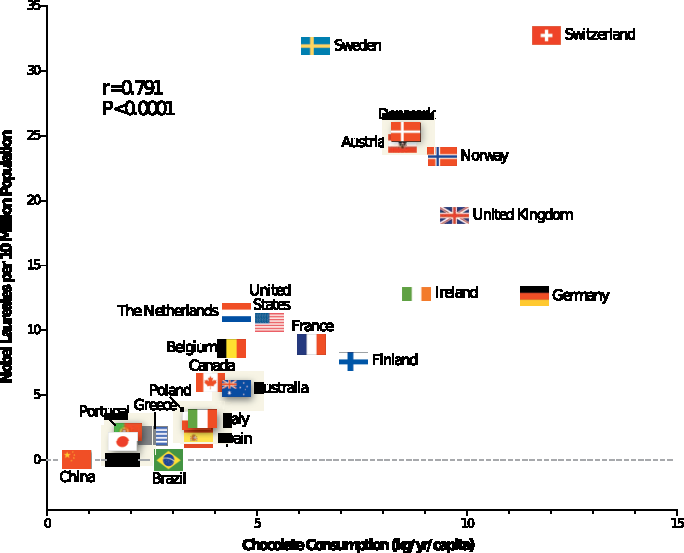
\includegraphics[width=\linewidth]{figures/chocolate-nobel}
  \caption{\label{fig:chocolate-nobel}
    From \parencite{messerli2012}.
    The figure shows a strong correlation between chocolate consumption
    in a country and number of Nobel prizes awarded to its citizens.
  }
\end{marginfigure}
A more scientific example is the unmistakeable correlation
shown in Figure~\ref{fig:chocolate-nobel}
between per-capita chocolate consumption
and number of Nobel laureates in a country.
Although the correlation is sound,
you should think twice before going into a chocolate diet
with the hope of winning a Nobel prize.

Another issue is that statistical dependence (correlation)
does not indicate the direction of the causation.
For example,
for a bystander observing a fire,
it may seem like `as more fire trucks arrive, the fire gets worse',
but the direction of causation is probably the other way around.
So although,
we won't be doing any analysis of causation,
you've been warned for this common error
(see also the cartoon in Figure~\ref{fig:xkcd-correlation}).
\begin{figure}
  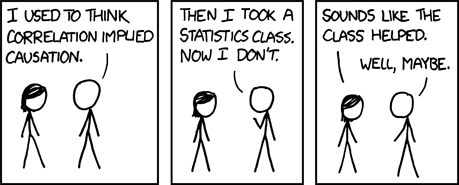
\includegraphics[width=\linewidth]{figures/xkcd-correlation}
  \caption{\url{http://xkcd.com/552/}}\label{fig:xkcd-correlation}%
\end{figure}

% TODO: multi-variate Gaussian?


\section{Where do the probabilities come from?}

So far,
we treated probabilities as numbers (between 0 and 1, inclusive)
and did not say much about where do they come from.
The question of what exactly a probability is a difficult one, 
and there have been (rival) alternative views on it.
Two well-known views,
we will encounter often is \emph{frequentist} (classical)
and \emph{Bayesian} (probabilistic) approaches.
Although both share all the aspects of probability theory we discussed above,
the interpretations of probability in these views differ,
and often lead to different methods for estimating probabilities.
This section is an informal, rather `philosophical', note on this difference.
We will frequently return to it later in this course.

In frequentist view,
the notion of probability is related to long-run relative frequency.
That is,
probability of an event is relative frequency of its occurrence.
For example,
if we are interested in probability of a particular word,
we can find it's relative frequency on a large corpus.
That is,
the number of times the word we are interested in appears in the corpus
divided by the number of words in the corpus.
Frequency-based probabilities leads to the estimation method called
\emph{maximum likelihood estimation} (MLE) we will discuss later.
% TODO: when/where?
The MLE is prevalent in statistics and machine learning.
As we will discuss in many places, however,
MLE \emph{overfits} the data it uses for the estimation,
the findings may not be general enough to be useful
outside the data used for estimation.
There are some modifications to MLE,
that makes it more resistant to overfitting.

In frequentist view of probability,
not every statement can be assigned to a probability value.
Some quantities we are often interested are fixed,
hence there is no notion of repeated experiments,
and hence, no probability value.
For example,
we can assign a probability value to
whether the next sentence in a speech (or in a book) will be
\num{10} words long.
Because this is a repeatable experiment.
However,
we cannot assign a probability value to average number of words
in a sentence in English (to simplify, say, in all written documents so far).
Even though we do not know this quantity,
there is a single number expressing it.
Hence, in frequentist view we cannot talk about,
the probability of average sentence length being \num{10}.
This seemingly `philosophical' standpoint has a very big impact
on how results are evaluated in experimental studies,
and hence, on the current scientific enterprise.

Intuitively,
frequency of an event and its probability is strongly related.
However,
our everyday notion of probability does
not necessarily involve repetitive experiments.
If you were given a fair coin,
you would not need a large number of experiments to conclude
that the probability of heads (or tails) is \num[round-precision=1]{0.5}.
On the practical side,
some events do not occur frequently enough to be estimated reliably.
As we will discuss at length in Chapter~\ref{chap:ngrams},
most objects of interest in NLP, such as words,
are particularly bad at showing up in where we look for them (in corpora).

The Bayesian notion of probability is based on (subjective)
`degree of belief',
matching more closely to our everyday notion of probability.
In this view,
probabilities are degrees of belief,
and updated `rationally',
with the data at hand based on rules of probability theory,
in particular based on the Bayes' formula we discussed in Section~\ref{sec:prob-bayes}.
Now that,
we consider probabilities as degrees of beliefs,
we can make probabilistic statements on things we are not allowed
in case of frequentist tradition.
For example,
we can easily talk about
the probability of average sentence length being \num{10},%
\footnote{Or, maybe between \num{9.5} and \num{10.5},
  since probabilities for single values is \num{0}
  for continuous random variables.}
and we can update this probability
(in fact the whole probability distribution) with the data we observe.
One particular benefit of the Bayesian estimation is that
we do not need anything other than probability theory for estimation.

A common criticism for Bayesian estimation is is that one needs to choose
a (subjective) prior probability (distribution)
before starting the data-driven estimation.
The word `subjective' does not sound like a good idea for science.
As a result,
Bayesian methods are often criticized for not being `objective'.
However, 
the prior information does not necessarily involve `personal' beliefs.
For example,
in our example with average number of words in a sentence,
there is nothing wrong to start with the presupposition that
the average number of sentences cannot be a negative number.
Further,
it is hardly a wrong assertion to assume that very large numbers,
e.g., \num{1000}, are very unlikely
(especially considering we are estimating \emph{average} sentence length).
There are many other forms of prior assumptions that are perfectly justified,
based on the knowledge accumulated in the field%
---often based on data from earlier studies.
Although making truly subjective decisions is not desirable
while interpreting experimental results in science,
if we shift our interest towards engineering rather than science,
the use of prior information (subjective or otherwise) is not
an issue at all.
There is nothing wrong with using a subjective method,
as long as it performs well for the task at hand.

A practical note on difference between the two estimation methods is
about the computational power required.
Bayesian estimation typically requires more computation power.
This difference is becoming less important
with the increasing power offered by developments in computer hardware
and approximate estimation techniques being developed.
However, it is still an important factor in many problems.

The debate is old and far from being settled yet.
In this course,
we do not take sides in this debate.
We introduce methods
that stem from both approaches for estimating probabilities.
The aim of this section is to inform the reader
about these different approaches
since they have important consequences for most of the methods we discuss.

% \section*{Where to go from here}
% 
% \textcite{grinstead2012} - online.
% 
% \textcite{mackay2003}
% 
% \textcite{jaynes2007}
